\chapter{Teste do Projecto}

Aqui demonstro o funcionamento do projecto, via testes a duas secções: a API e a interface. Para esta demonstração em cada uma das secções, vamos utilizar imagens representativas, tiradas através de \textit{PrintScreen}.

Qualquer teste começa sempre pelo \textit{Home} (o \textit{Index}).

\begin{figure}[!hbt]
    \centering
    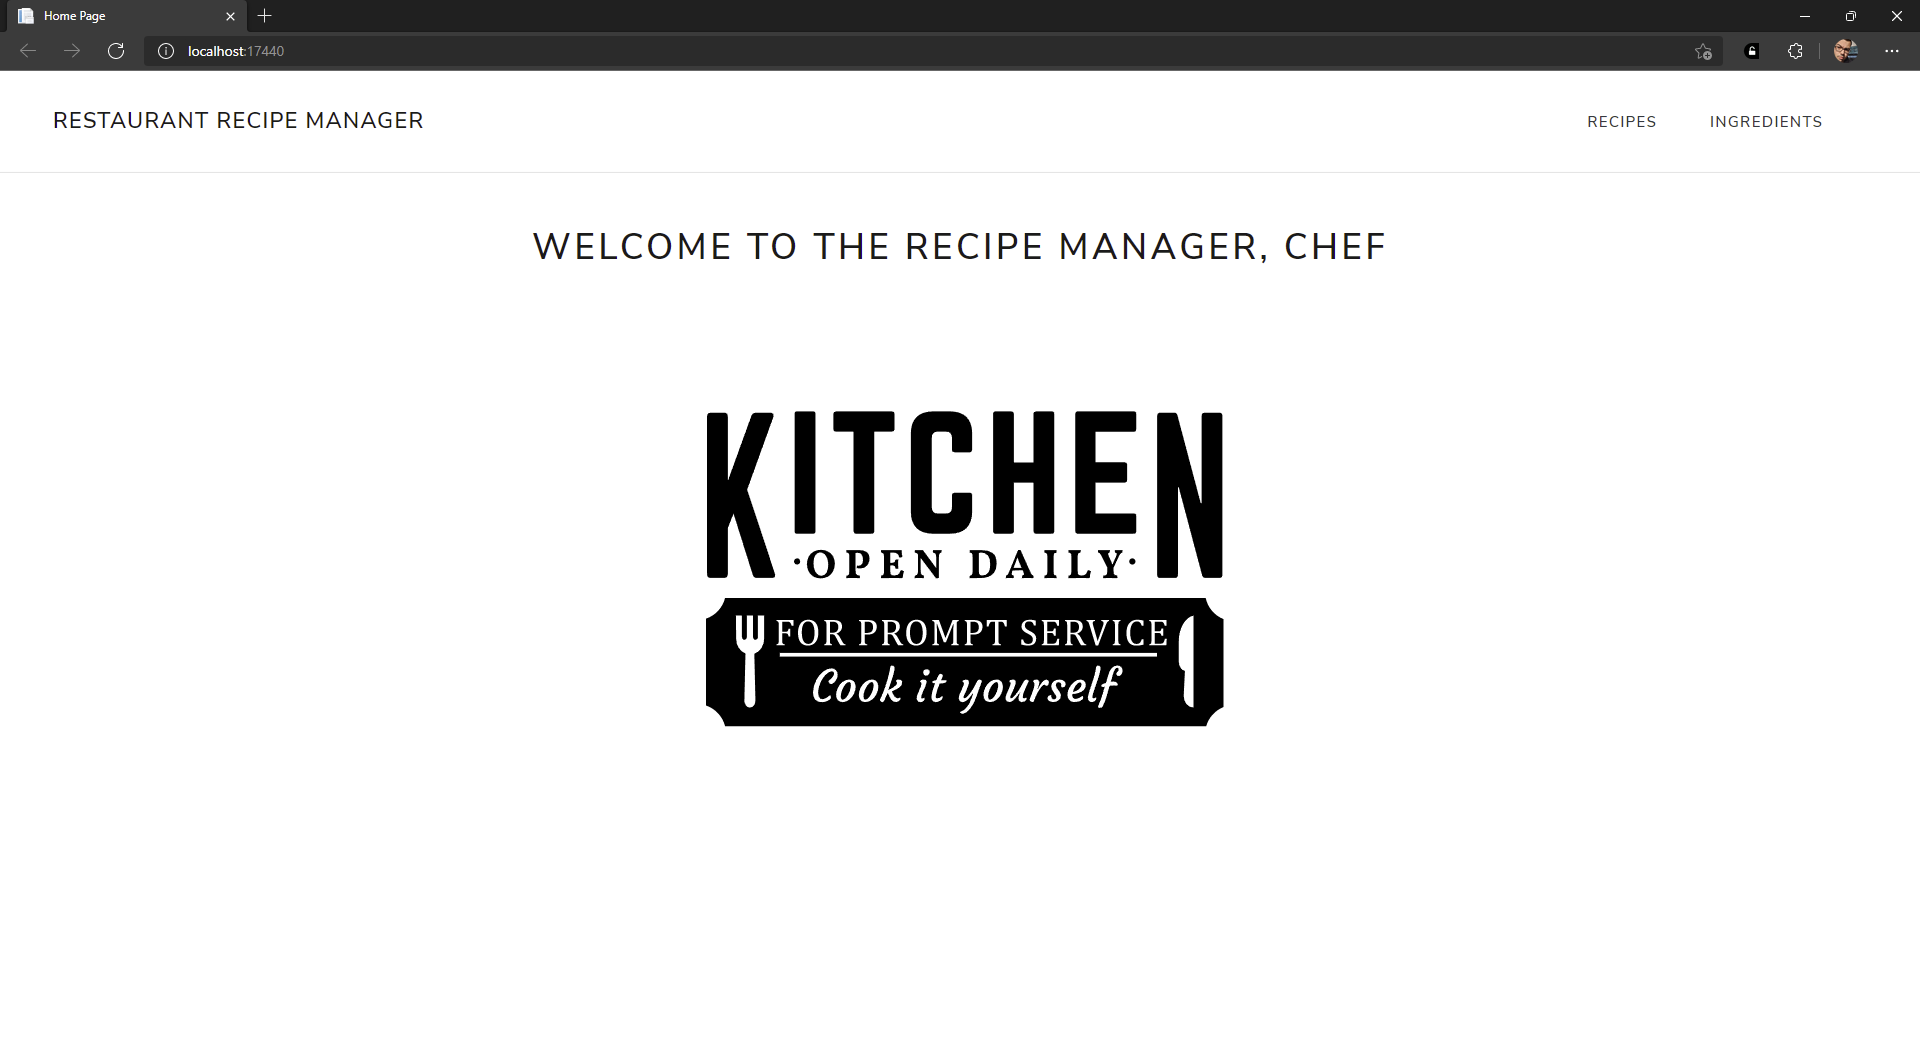
\includegraphics[width=14cm]{Resources/WebApp/Home/home.png}
    \caption{Ilustração do home da WebApp}
    
\end{figure}
\FloatBarrier

\section{Testes à API}

Para testar a API foi usado a extensão \textit{Thunder Client} do \textit{Visual Studio Code}. Esta é uma extensão que substitui o \textit{Postman}, que é um cliente HTTP que permite testar APIs.

Nas imagens seguintes podemos ver a API em funcionamento. O primeiro \textit{set} de imagens é referente ao caso de uso da Gestão de Ingredientes e Stock. O segundo referente ao caso de uso da Gestão de Receitas.

\newpage
\subsection{\textit{API/Ingredients}}

\begin{figure}[!hbt]
    \centering
    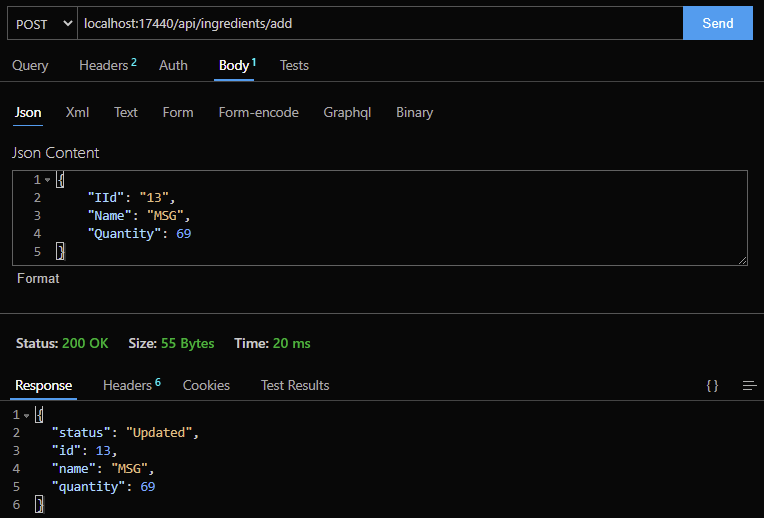
\includegraphics[width=14cm]{Resources/API/Ingredients/Ingredients (1).png}
    \caption{Ilustração do método POST a \textit{/api/ingredients/add}}
    
\end{figure}
\FloatBarrier
\begin{figure}[!hbt]
    \centering
    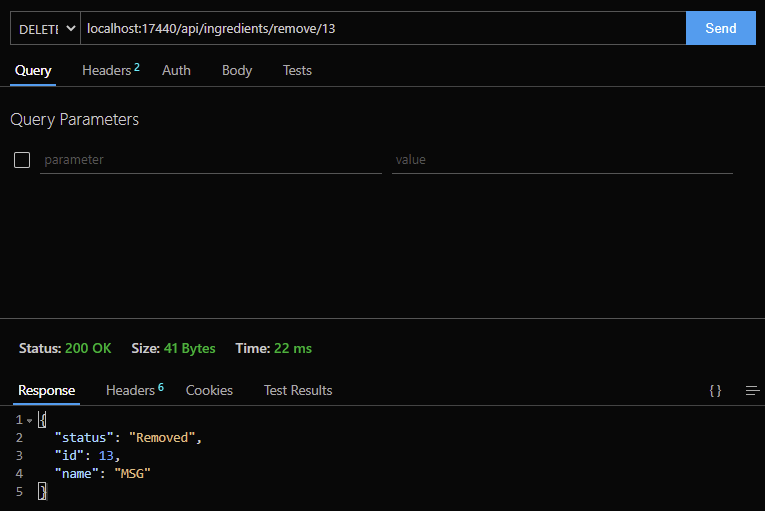
\includegraphics[width=14cm]{Resources/API/Ingredients/Ingredients (2).png}
    \caption{Ilustração do método DELETE a \textit{/api/remove/13}}
    
\end{figure}
\FloatBarrier
\begin{figure}[!hbt]
    \centering
    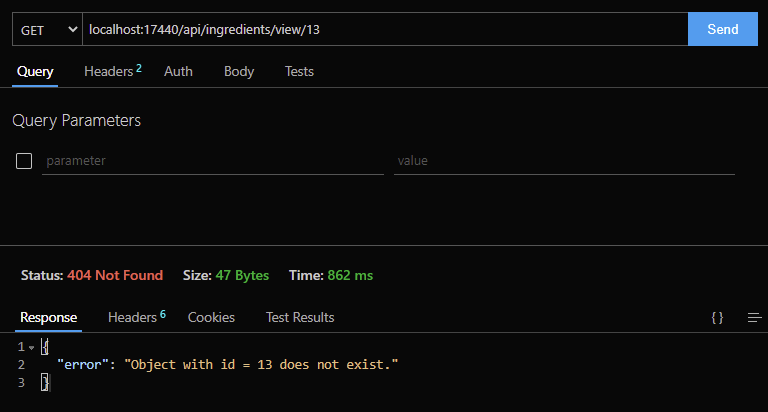
\includegraphics[width=14cm]{Resources/API/Ingredients/Ingredients (3).png}
    \caption{Ilustração do método GET a \textit{/api/ingredients/view/13}}
    
\end{figure}
\FloatBarrier
\begin{figure}[!hbt]
    \centering
    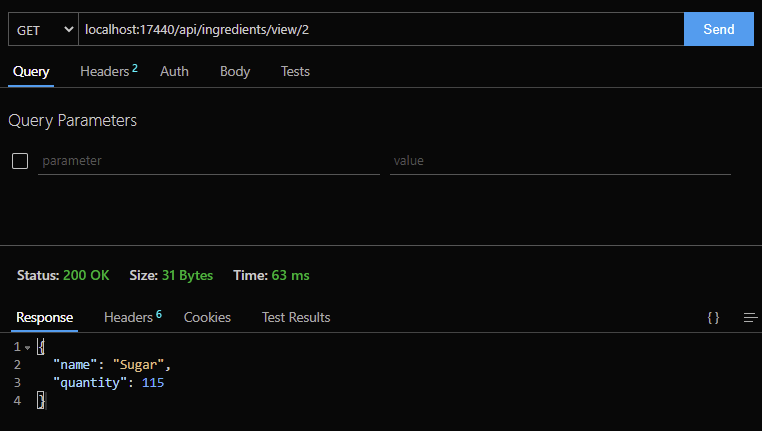
\includegraphics[width=14cm]{Resources/API/Ingredients/Ingredients (4).png}
    \caption{Ilustração do método GET a \textit{/api/ingredients/view/2}}
    
\end{figure}
\FloatBarrier
\begin{figure}[!hbt]
    \centering
    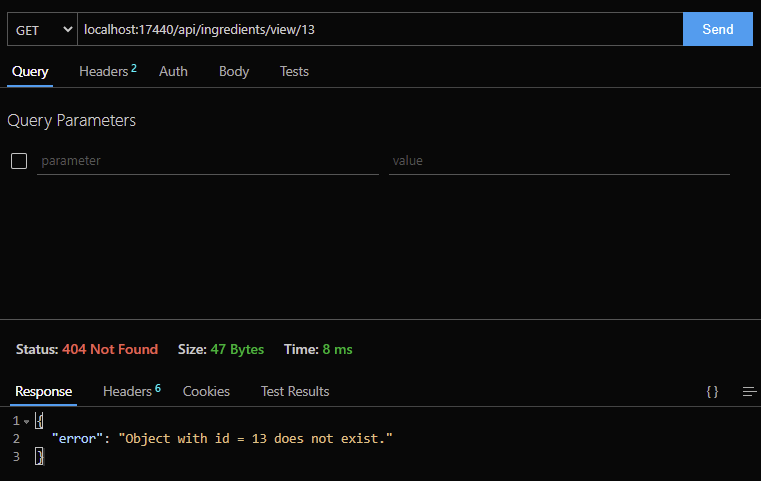
\includegraphics[width=14cm]{Resources/API/Ingredients/Ingredients (5).png}
    \caption{Ilustração do método GET a \textit{/api/ingredients/view/13}}
    
\end{figure}
\FloatBarrier
\begin{figure}[!hbt]
    \centering
    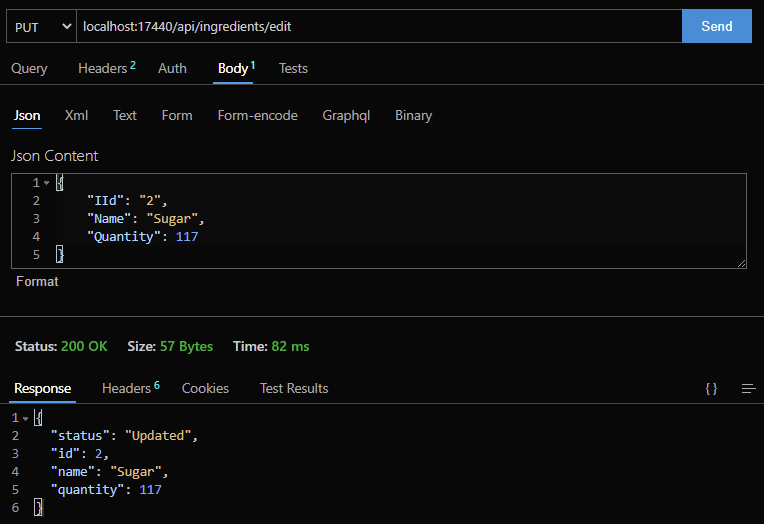
\includegraphics[width=14cm]{Resources/API/Ingredients/Ingredients (6).png}
    \caption{Ilustração do método PUT a \textit{/api/ingredients/edit}}
    
\end{figure}
\FloatBarrier
\begin{figure}[!hbt]
    \centering
    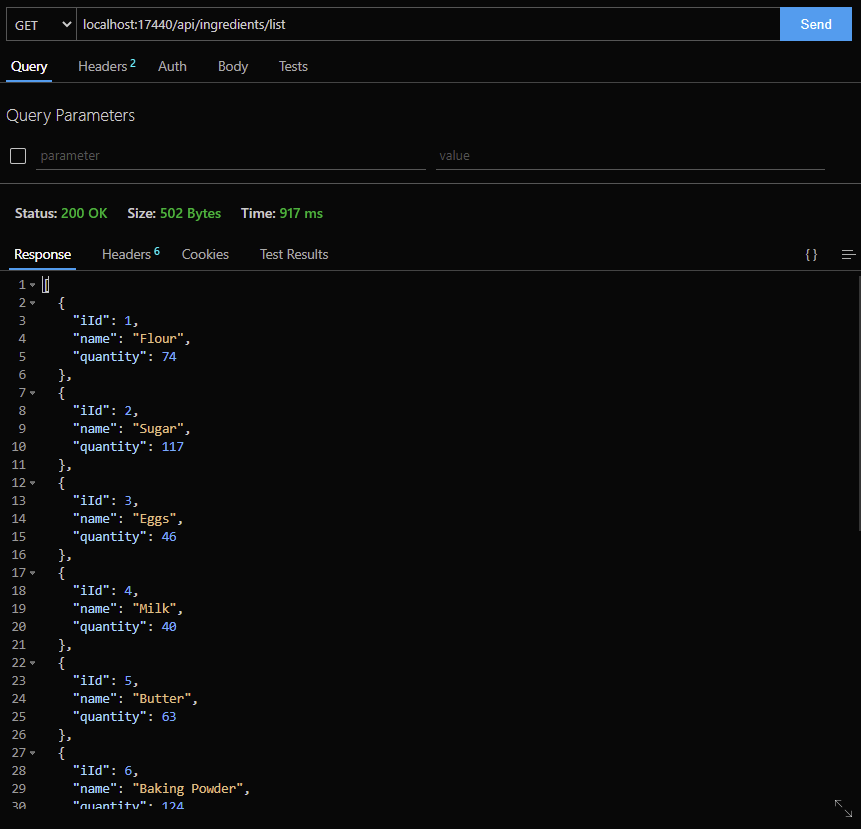
\includegraphics[width=14cm]{Resources/API/Ingredients/Ingredients (7).png}
    \caption{Ilustração do método GET a \textit{/api/ingredients/list}}
    
\end{figure}
\FloatBarrier
\begin{figure}[!hbt]
    \centering
    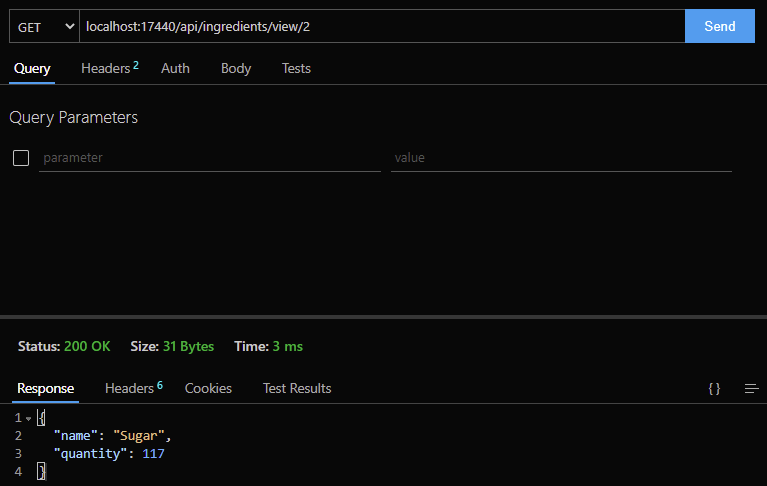
\includegraphics[width=14cm]{Resources/API/Ingredients/Ingredients (8).png}
    \caption{Ilustração do método GET a \textit{/api/ingredients/view/2}}
    
\end{figure}
\FloatBarrier

\newpage
\subsection{\textit{API/Recipes}}

\begin{figure}[!hbt]
    \centering
    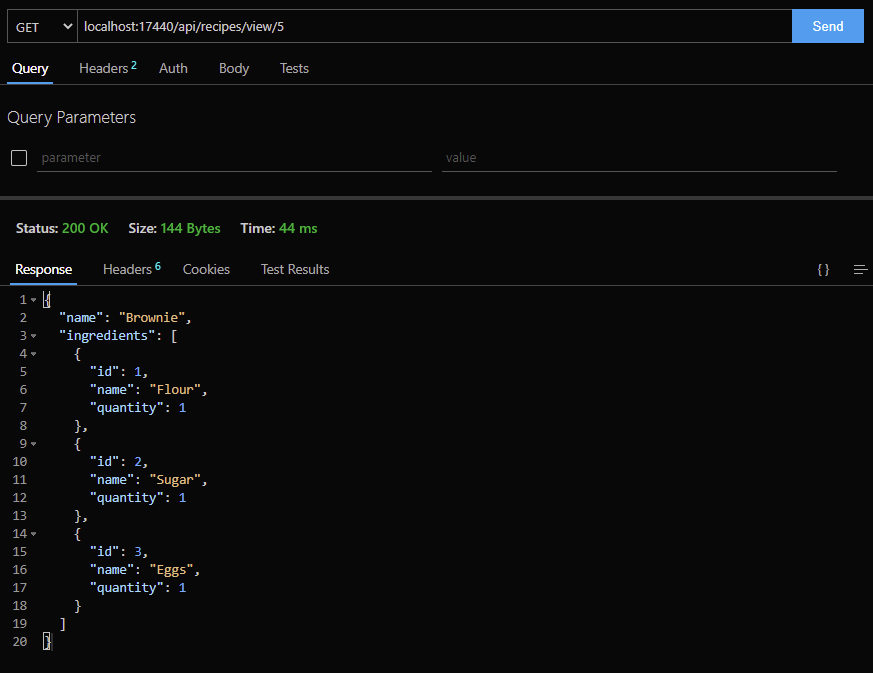
\includegraphics[width=14cm]{Resources/API/Recipes/Recipes (1).png}
    \caption{Ilustração do método GET a \textit{/api/recipes/view/5}}
    
\end{figure}
\FloatBarrier
\begin{figure}[!hbt]
    \centering
    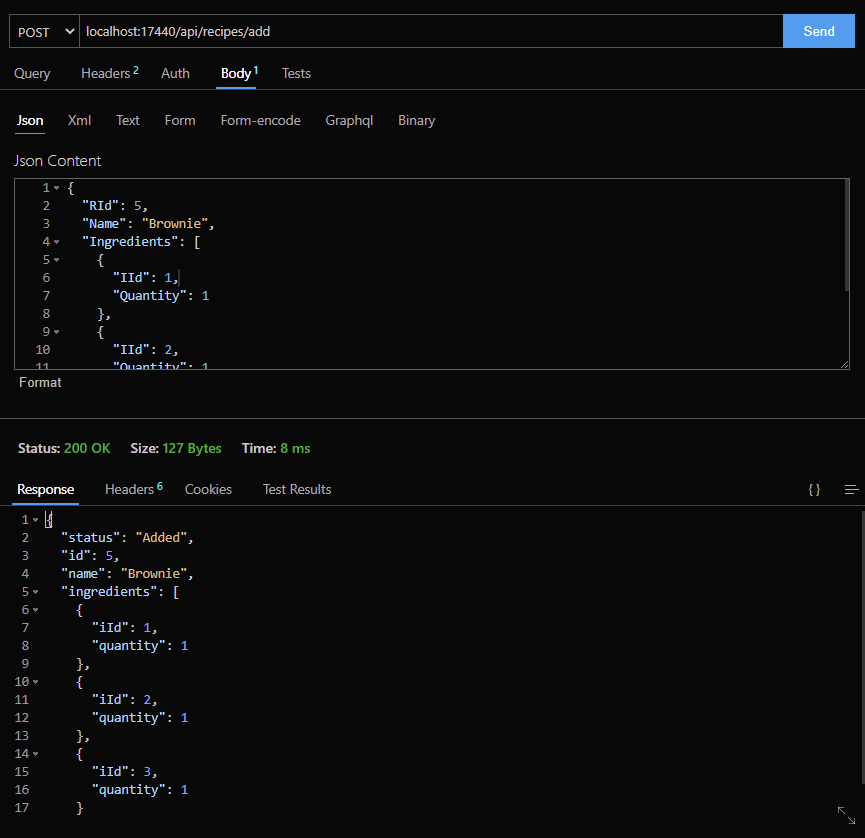
\includegraphics[width=14cm]{Resources/API/Recipes/Recipes (2).png}
    \caption{Ilustração do método POST a \textit{/api/recipes/add}}
    
\end{figure}
\FloatBarrier
\begin{figure}[!hbt]
    \centering
    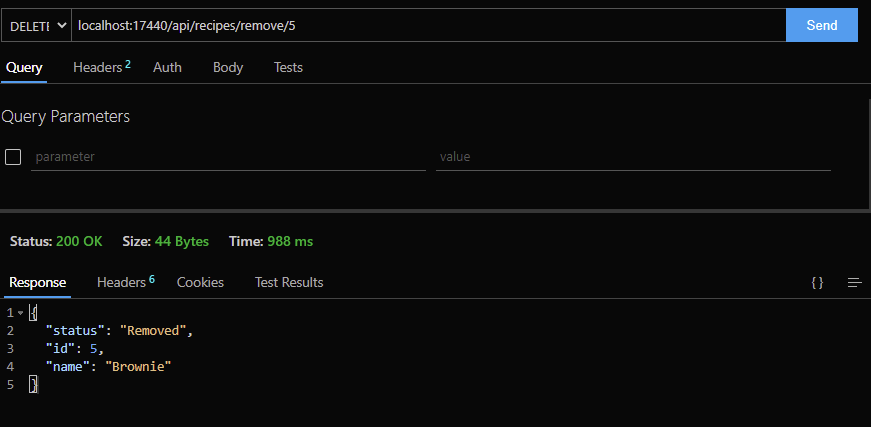
\includegraphics[width=14cm]{Resources/API/Recipes/Recipes (3).png}
    \caption{Ilustração do método DELETE a \textit{/api/recipes/remove/5}}
    
\end{figure}
\FloatBarrier
\begin{figure}[!hbt]
    \centering
    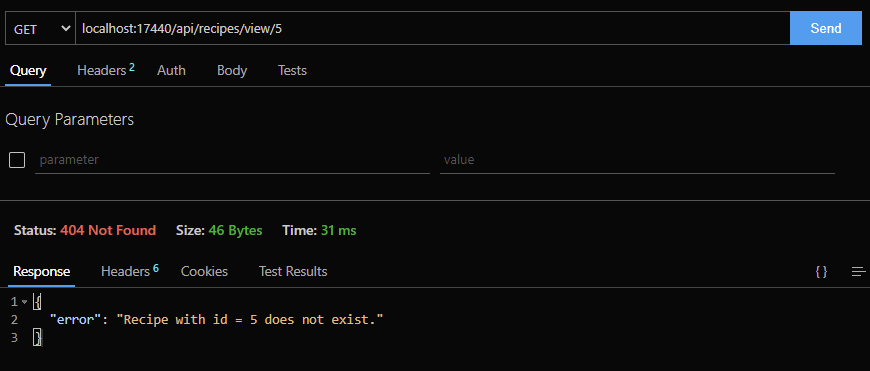
\includegraphics[width=14cm]{Resources/API/Recipes/Recipes (4).png}
    \caption{Ilustração do método GET a \textit{/api/recipes/view/5}}
    
\end{figure}
\FloatBarrier
\begin{figure}[!hbt]
    \centering
    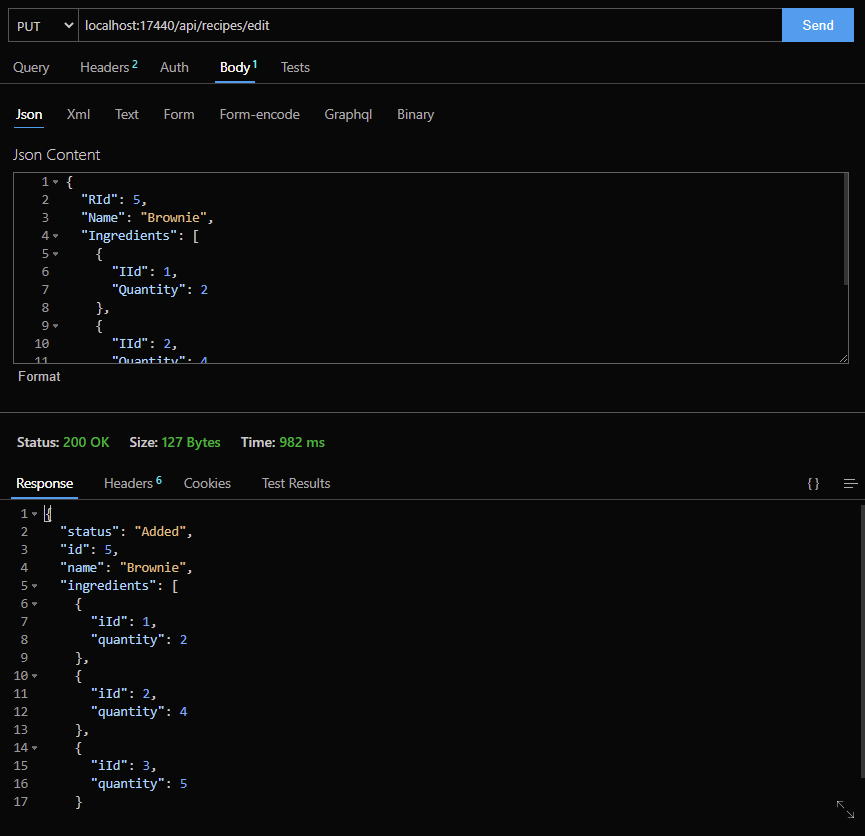
\includegraphics[width=14cm]{Resources/API/Recipes/Recipes (5).png}
    \caption{Ilustração do método PUT a \textit{/api/recipes/edit}}
    
\end{figure}
\FloatBarrier
\begin{figure}[!hbt]
    \centering
    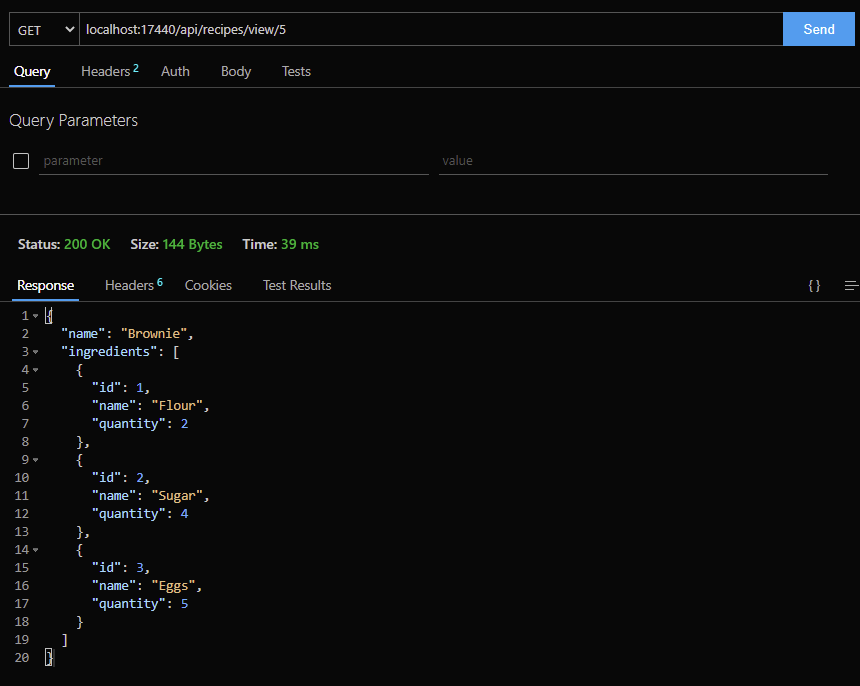
\includegraphics[width=14cm]{Resources/API/Recipes/Recipes (6).png}
    \caption{Ilustração do método GET a \textit{/api/recipes/view/5}}
    
\end{figure}
\FloatBarrier
\begin{figure}[!hbt]
    \centering
    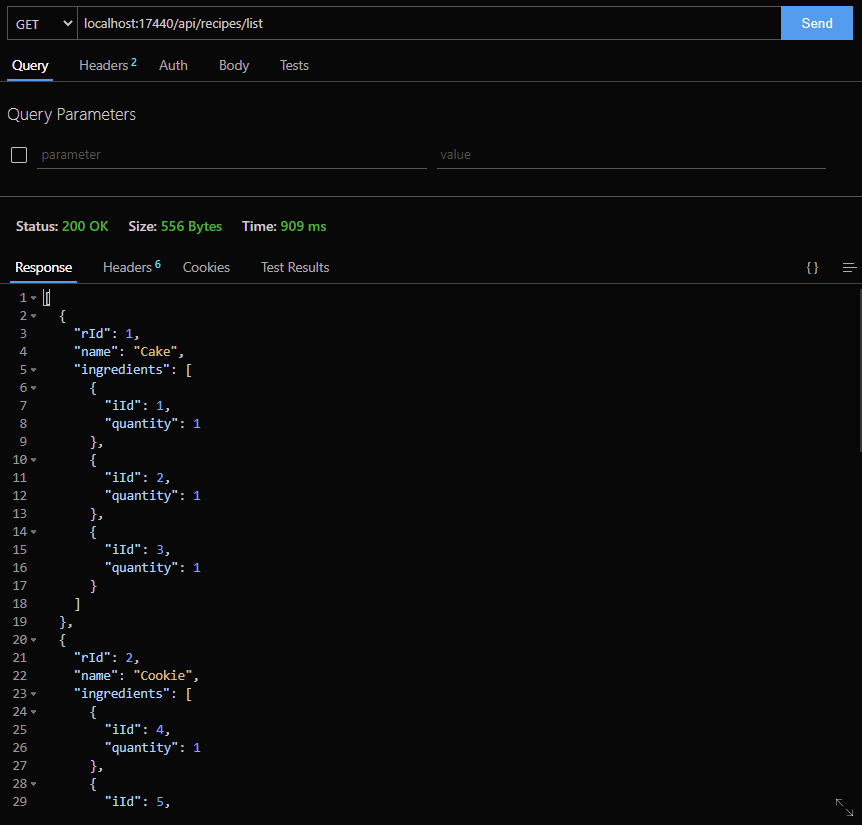
\includegraphics[width=14cm]{Resources/API/Recipes/Recipes (7).png}
    \caption{Ilustração do método GET a \textit{/api/recipes/list}}
    
\end{figure}
\FloatBarrier

\newpage
\section{Testes a Aplicação Web}

A aplicação web foi testada através do navegador Edge (Chromium). O qual podemos ver nas imagens seguintes.

Nestes dois \textit{sets} de imagens, podemos confirmar o funcionamento da aplicação web. O primeiro é referente ao caso de uso da Gestão de Ingredientes e Stock. O segundo referente ao caso de uso da Gestão de Receitas.

\subsection{\textit{Ingredient}}

\begin{figure}[!hbt]
    \centering
    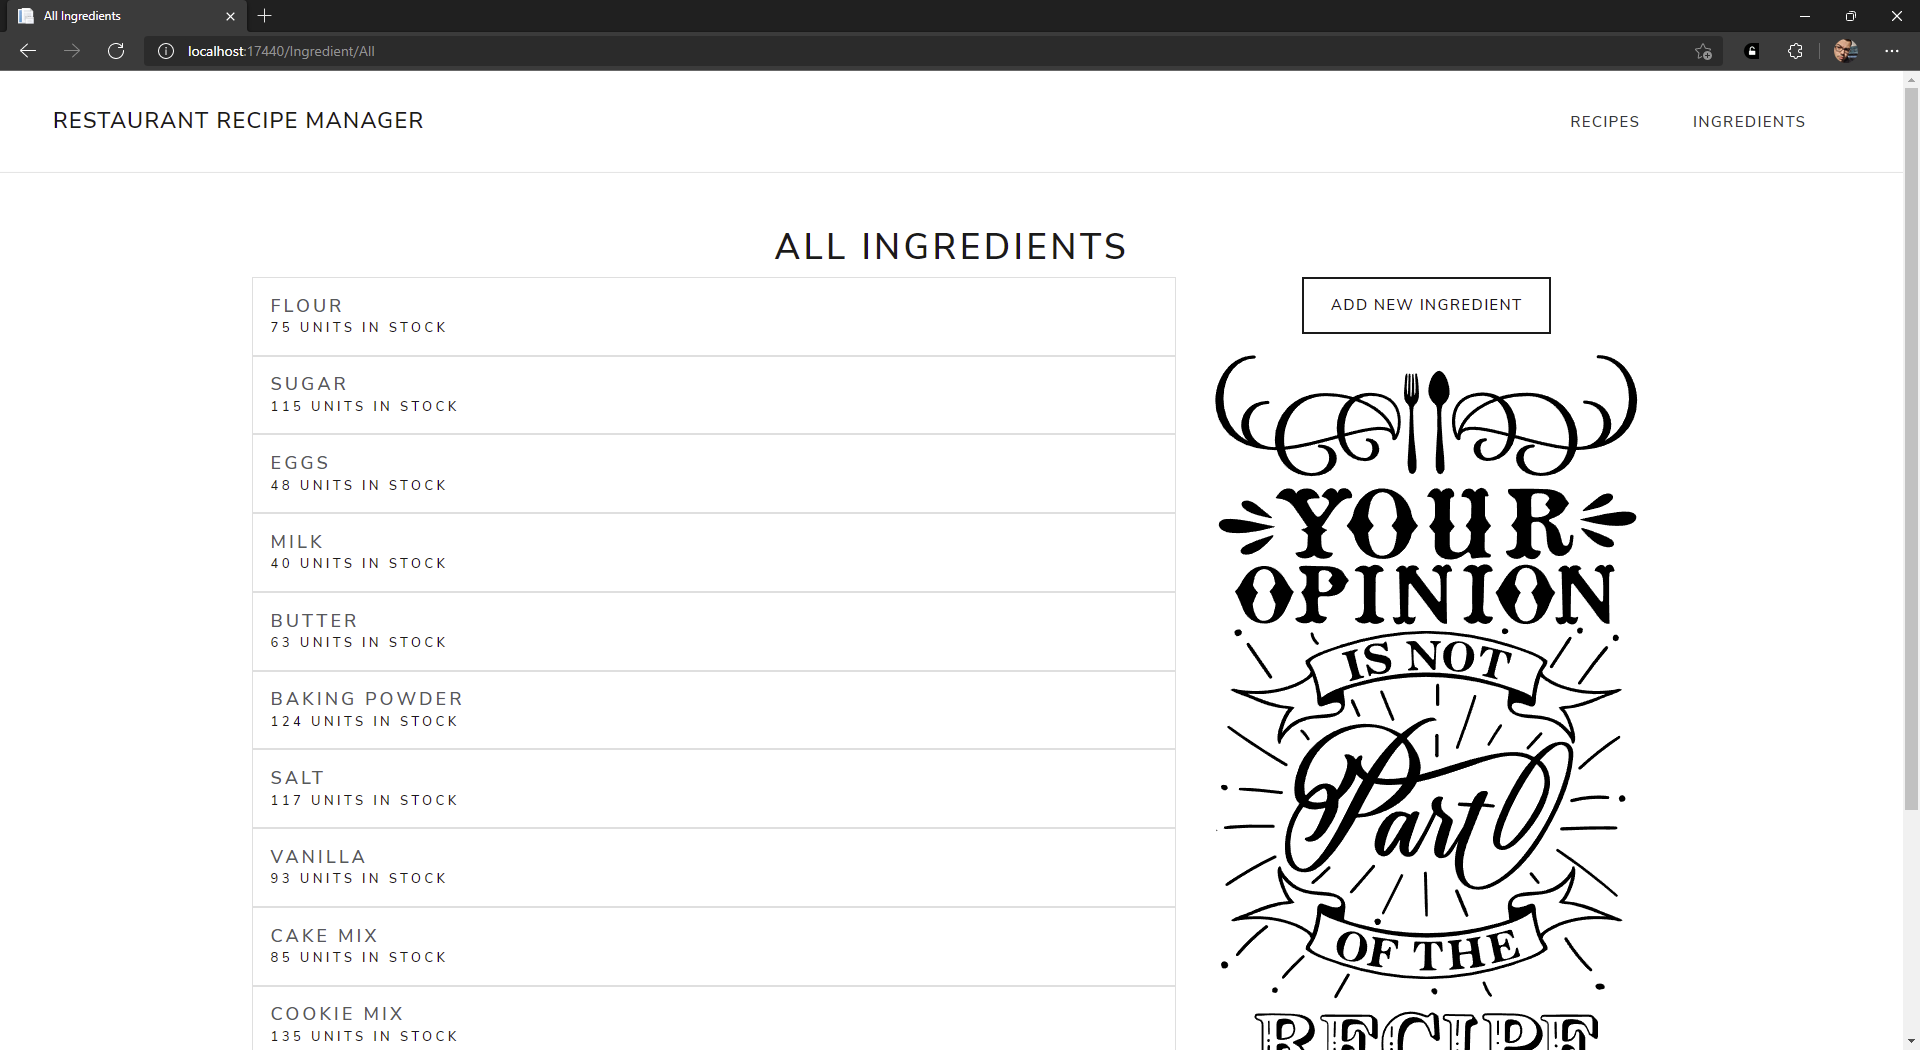
\includegraphics[width=14cm]{Resources/WebApp/Ingredients/ingredient (1).png}
    \caption{Ilustração da lista de Ingredientes}
    
\end{figure}
\FloatBarrier
\begin{figure}[!hbt]
    \centering
    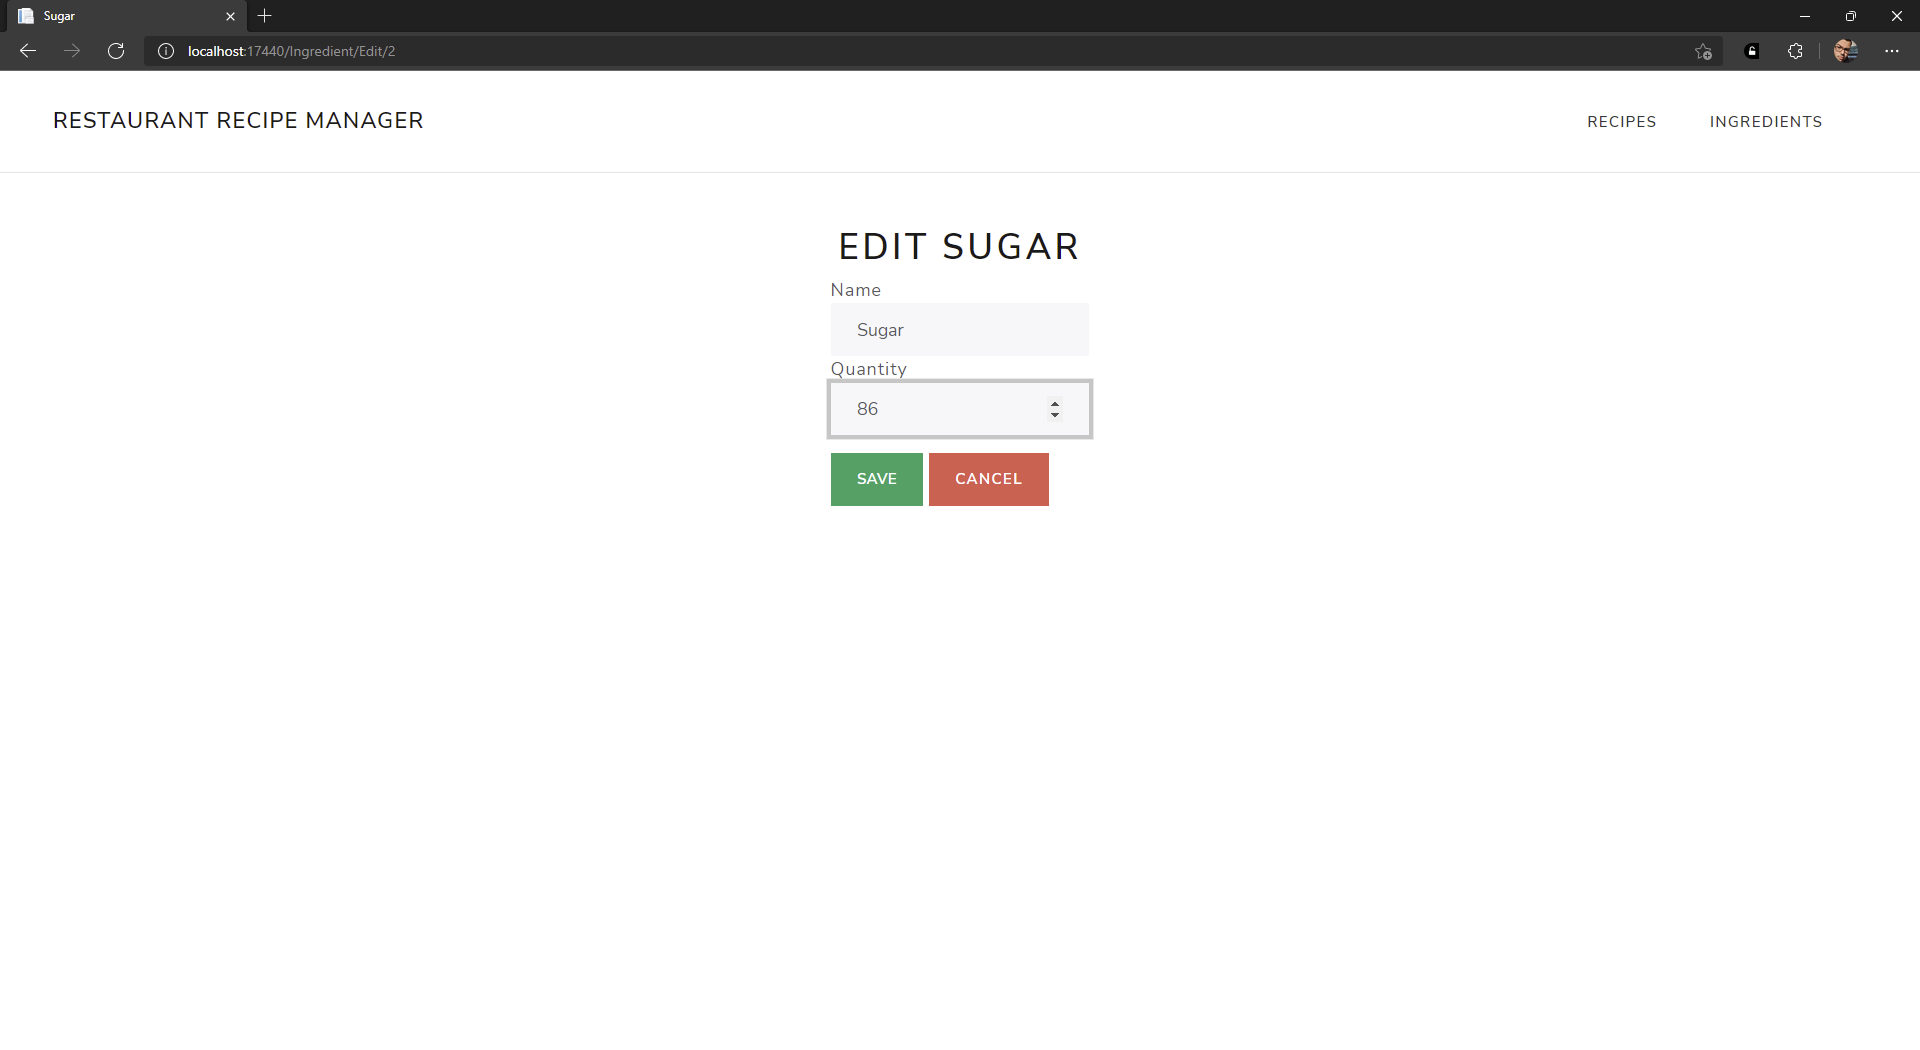
\includegraphics[width=14cm]{Resources/WebApp/Ingredients/ingredient (2).png}
    \caption{Ilustração da edição do Açúcar}
    
\end{figure}
\FloatBarrier
\begin{figure}[!hbt]
    \centering
    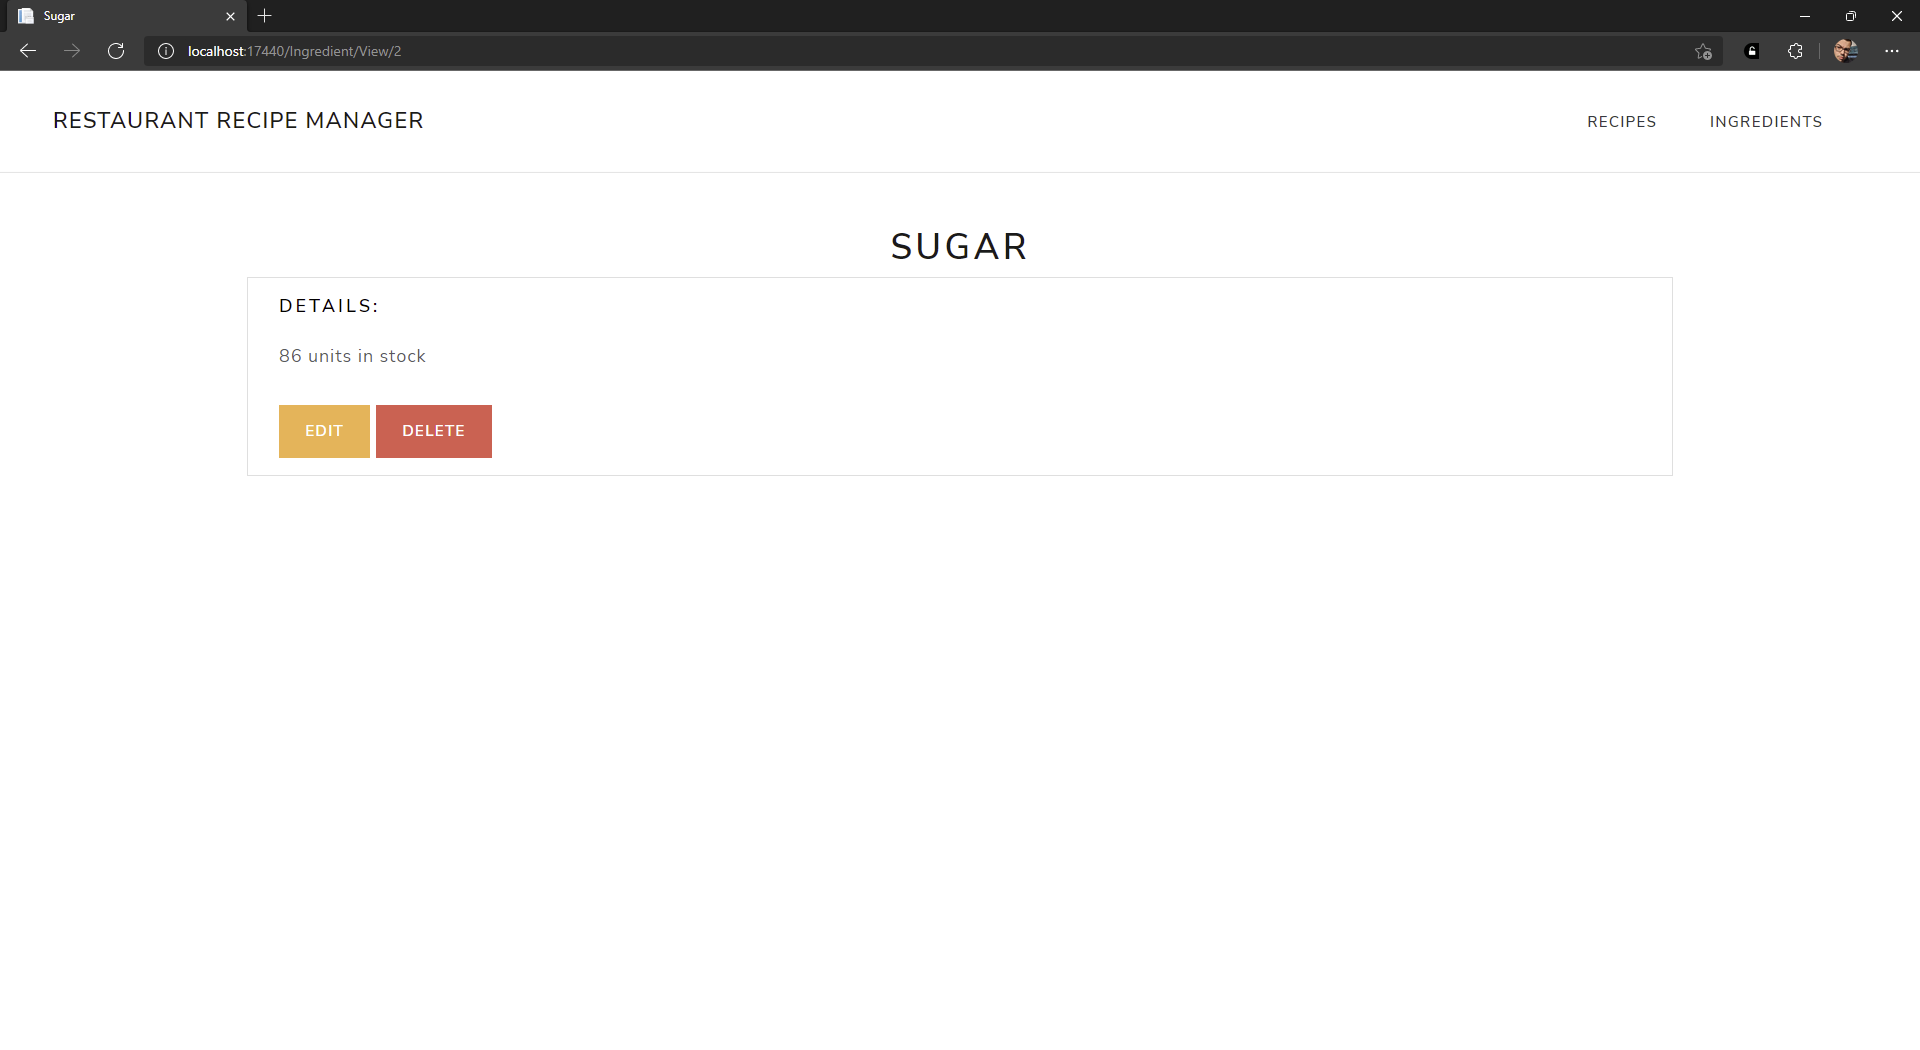
\includegraphics[width=14cm]{Resources/WebApp/Ingredients/ingredient (3).png}
    \caption{Ilustração da mostra do Açúcar pós alteração}
    
\end{figure}
\FloatBarrier
\begin{figure}[!hbt]
    \centering
    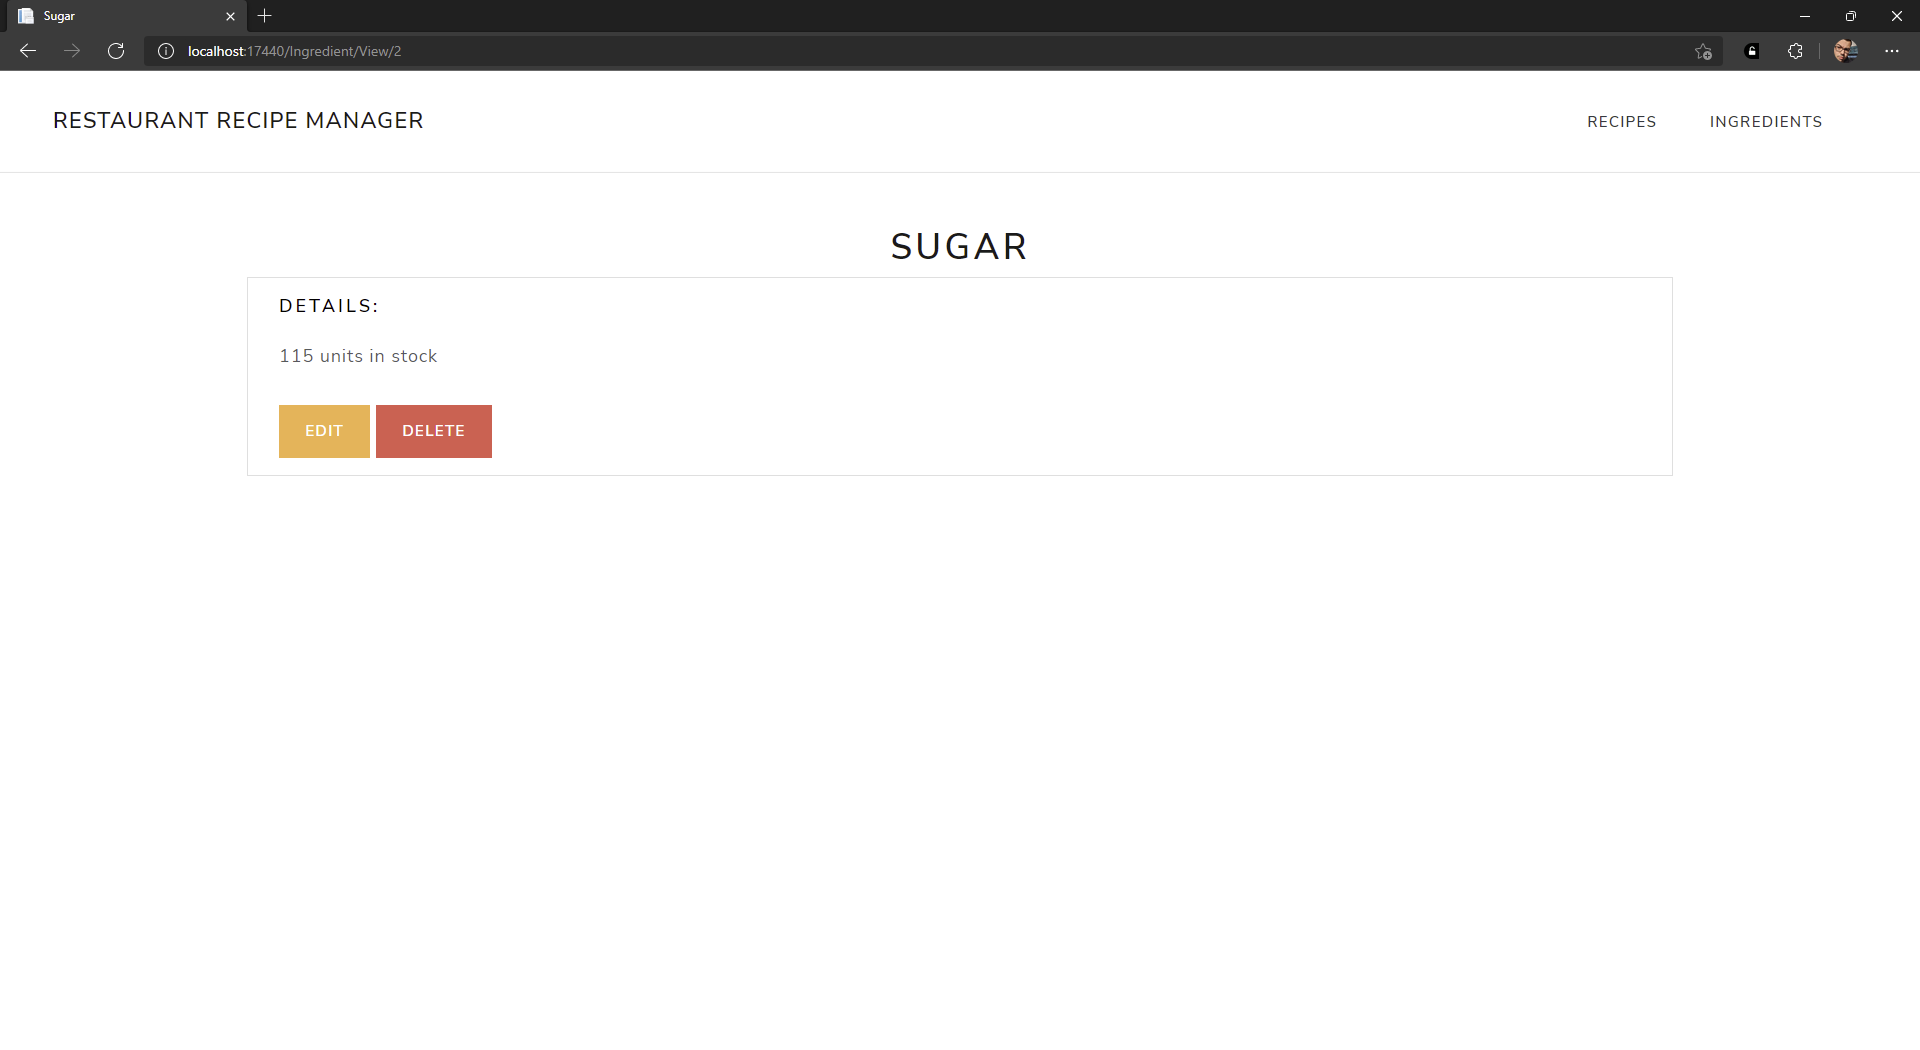
\includegraphics[width=14cm]{Resources/WebApp/Ingredients/ingredient (4).png}
    \caption{Ilustração da mostra do Açúcar pré alteração}
    
\end{figure}
\FloatBarrier
\begin{figure}[!hbt]
    \centering
    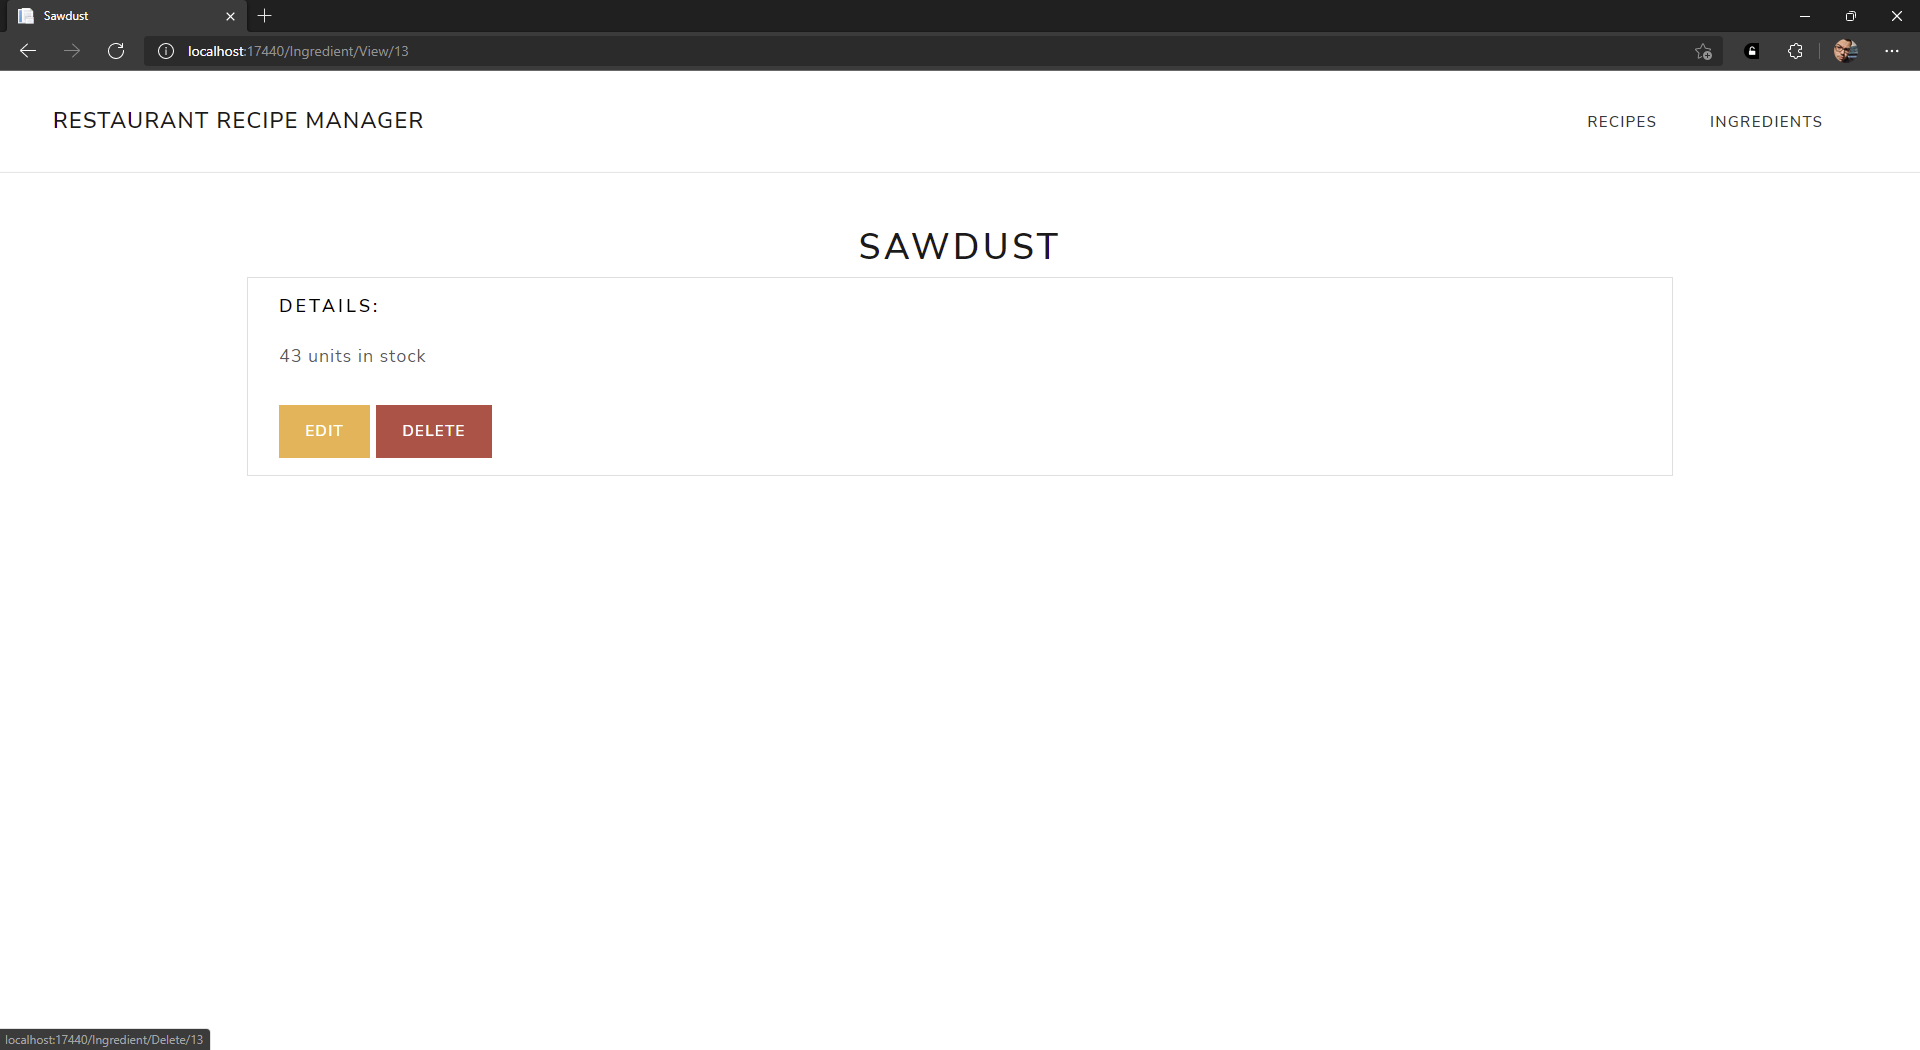
\includegraphics[width=14cm]{Resources/WebApp/Ingredients/ingredient (5).png}
    \caption{Ilustração da mostra da Serragem pré eliminação}
    
\end{figure}
\FloatBarrier
\begin{figure}[!hbt]
    \centering
    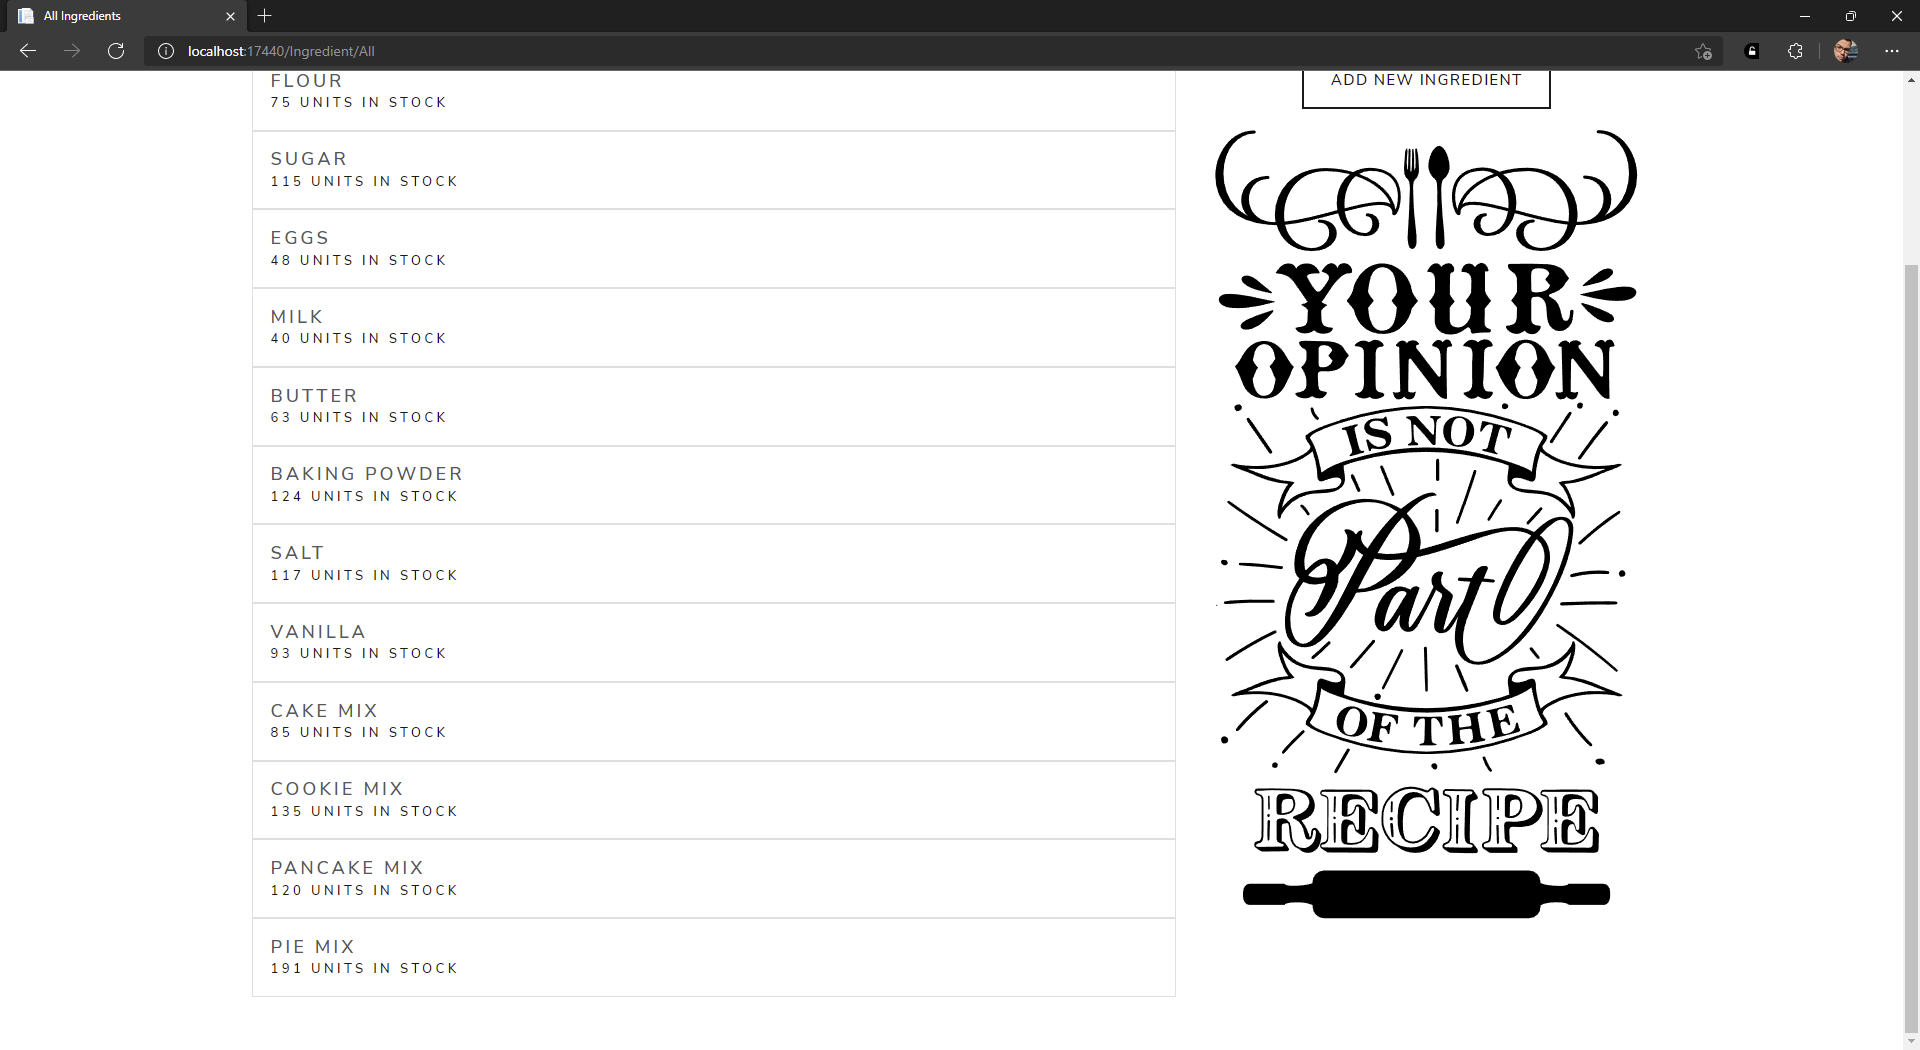
\includegraphics[width=14cm]{Resources/WebApp/Ingredients/ingredient (6).png}
    \caption{Ilustração da lista sem a Serragem}
    
\end{figure}
\FloatBarrier
\begin{figure}[!hbt]
    \centering
    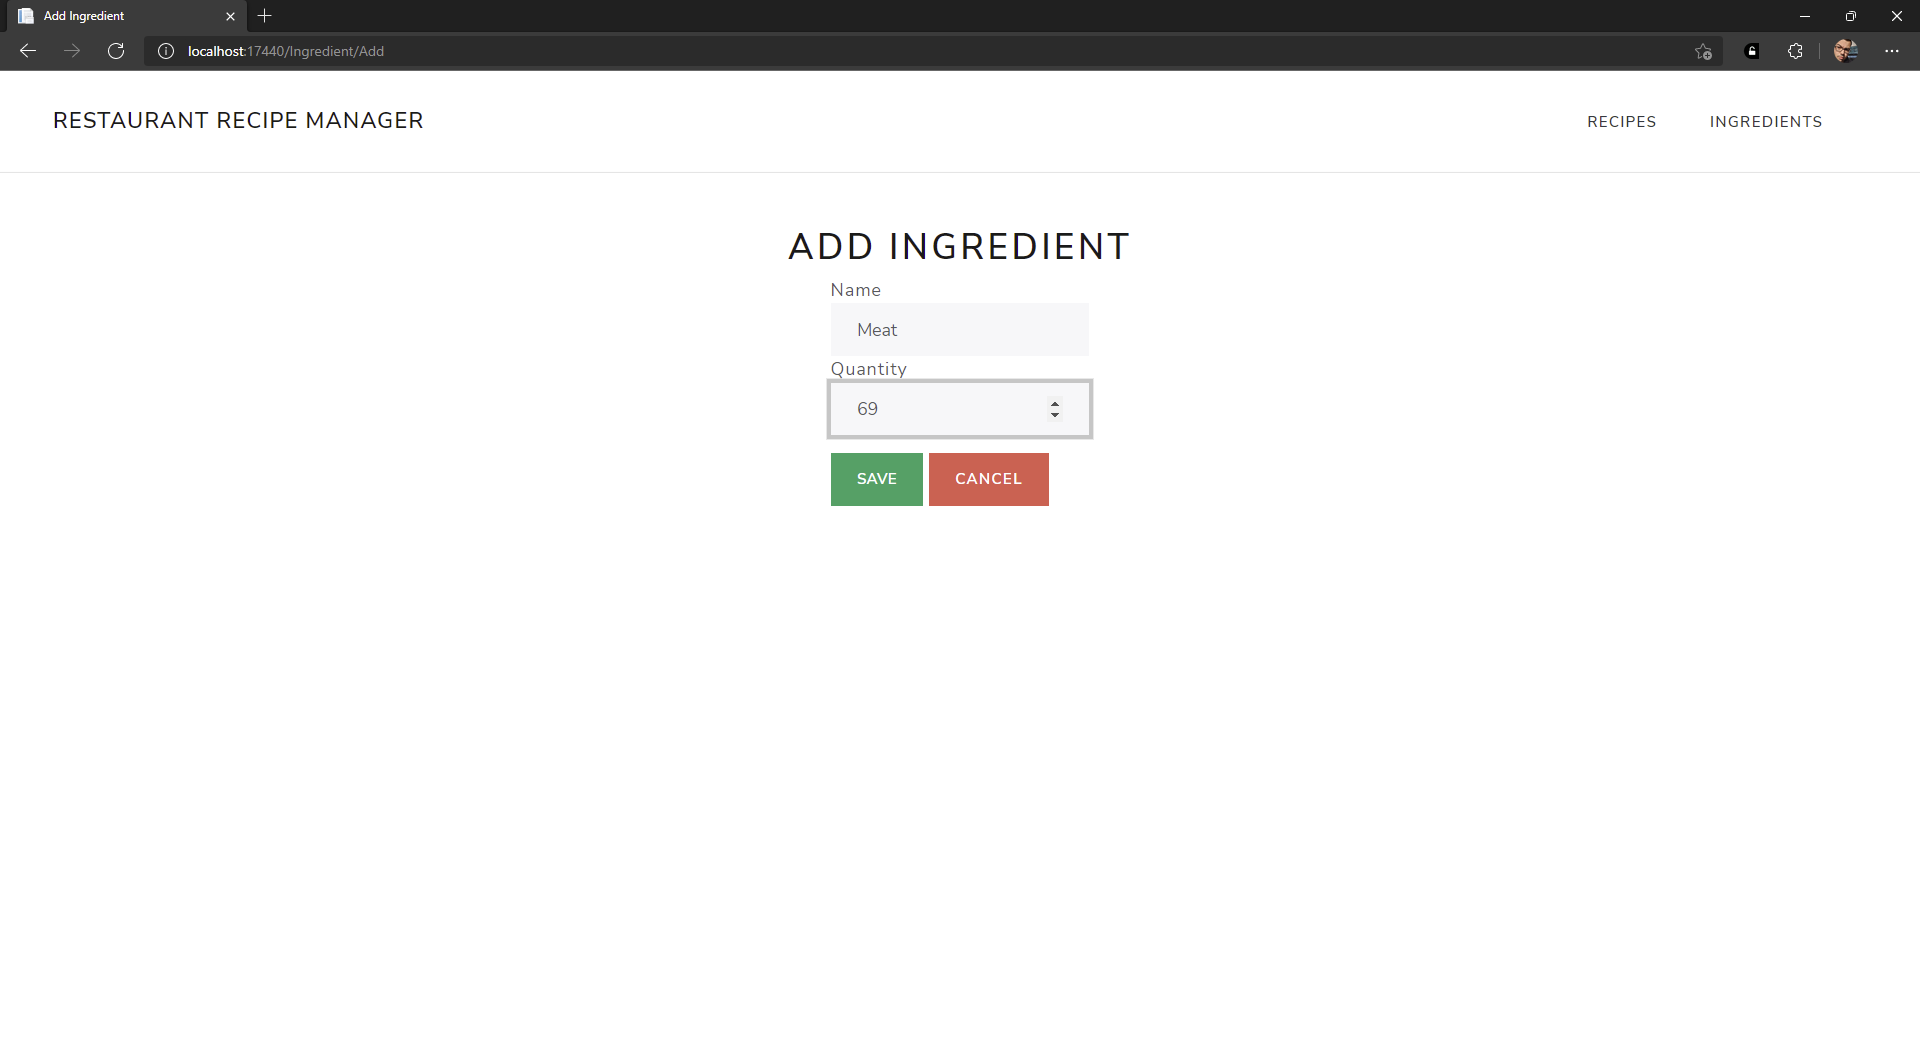
\includegraphics[width=14cm]{Resources/WebApp/Ingredients/ingredient (7).png}
    \caption{Ilustração da adição de Carne}
    
\end{figure}
\FloatBarrier
\begin{figure}[!hbt]
    \centering
    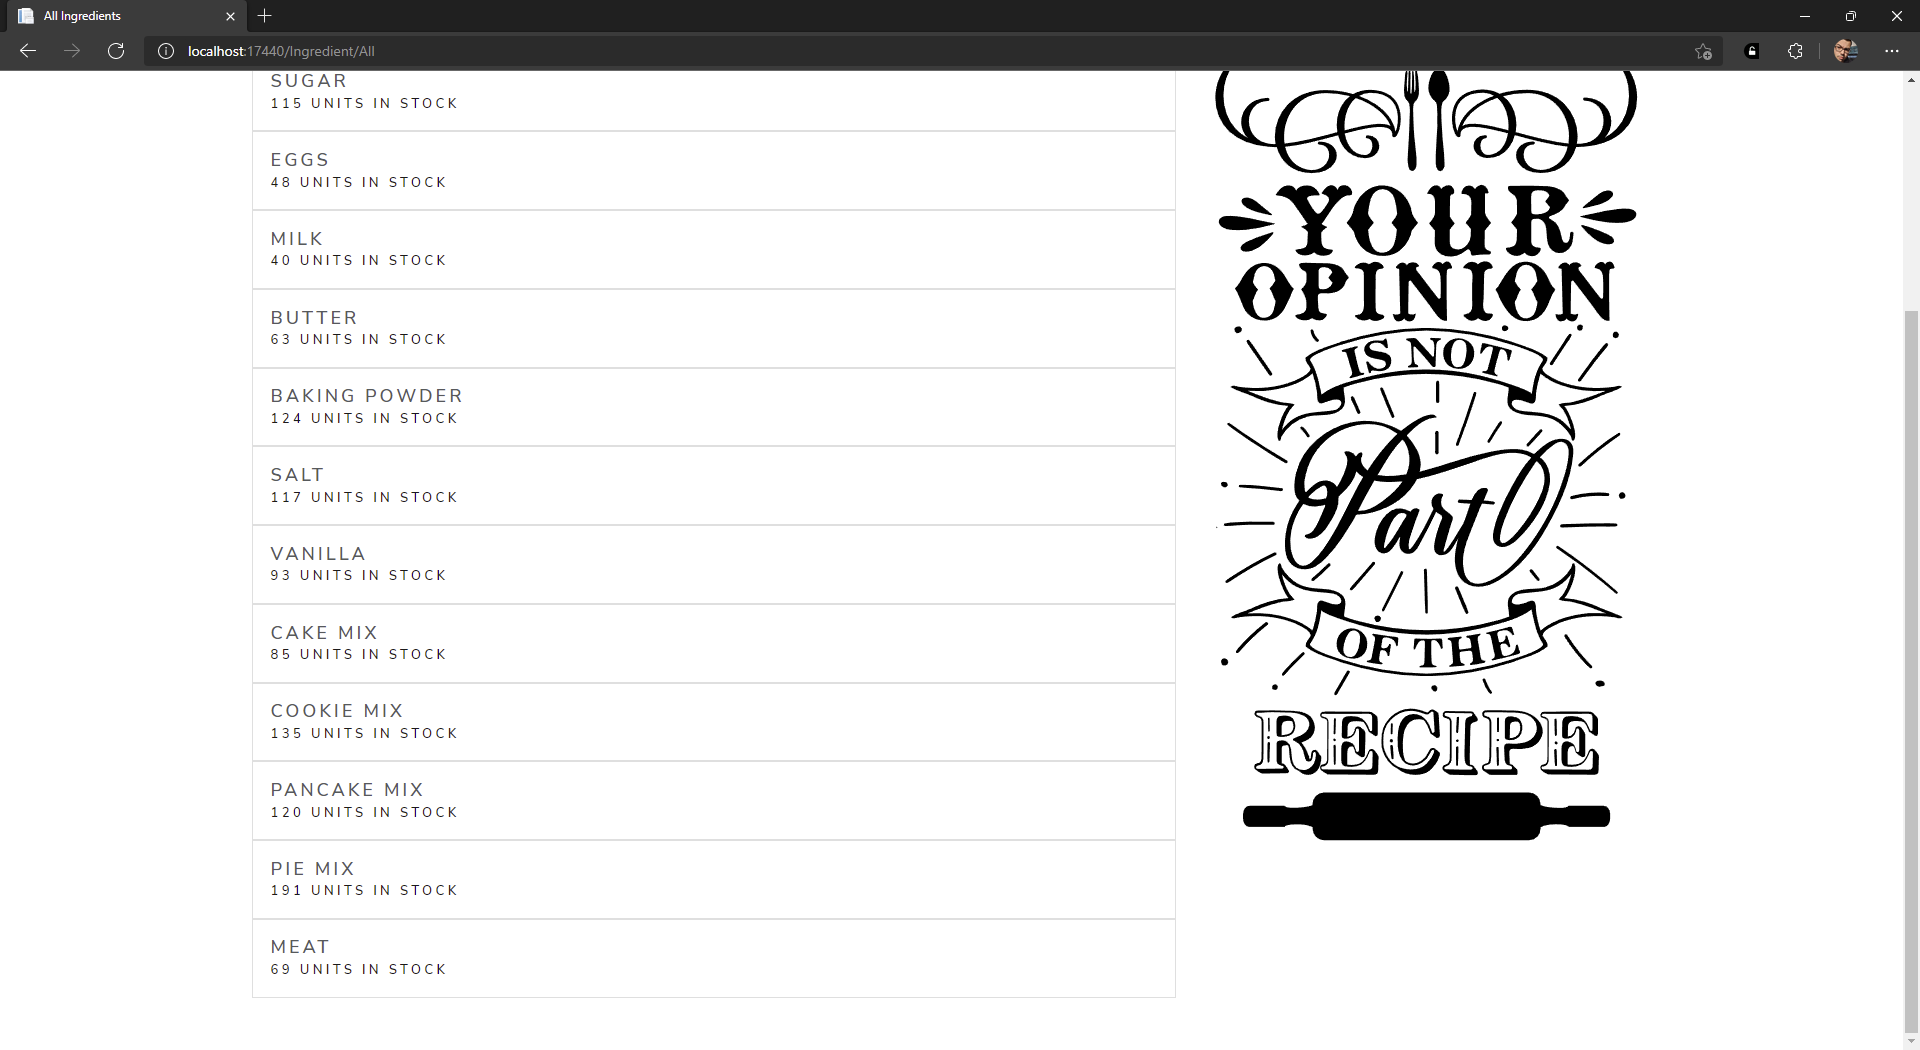
\includegraphics[width=14cm]{Resources/WebApp/Ingredients/ingredient (8).png}
    \caption{Ilustração da lista com Carne}
    
\end{figure}
\FloatBarrier

\newpage
\subsection{\textit{Recipe}}

\begin{figure}[!hbt]
    \centering
    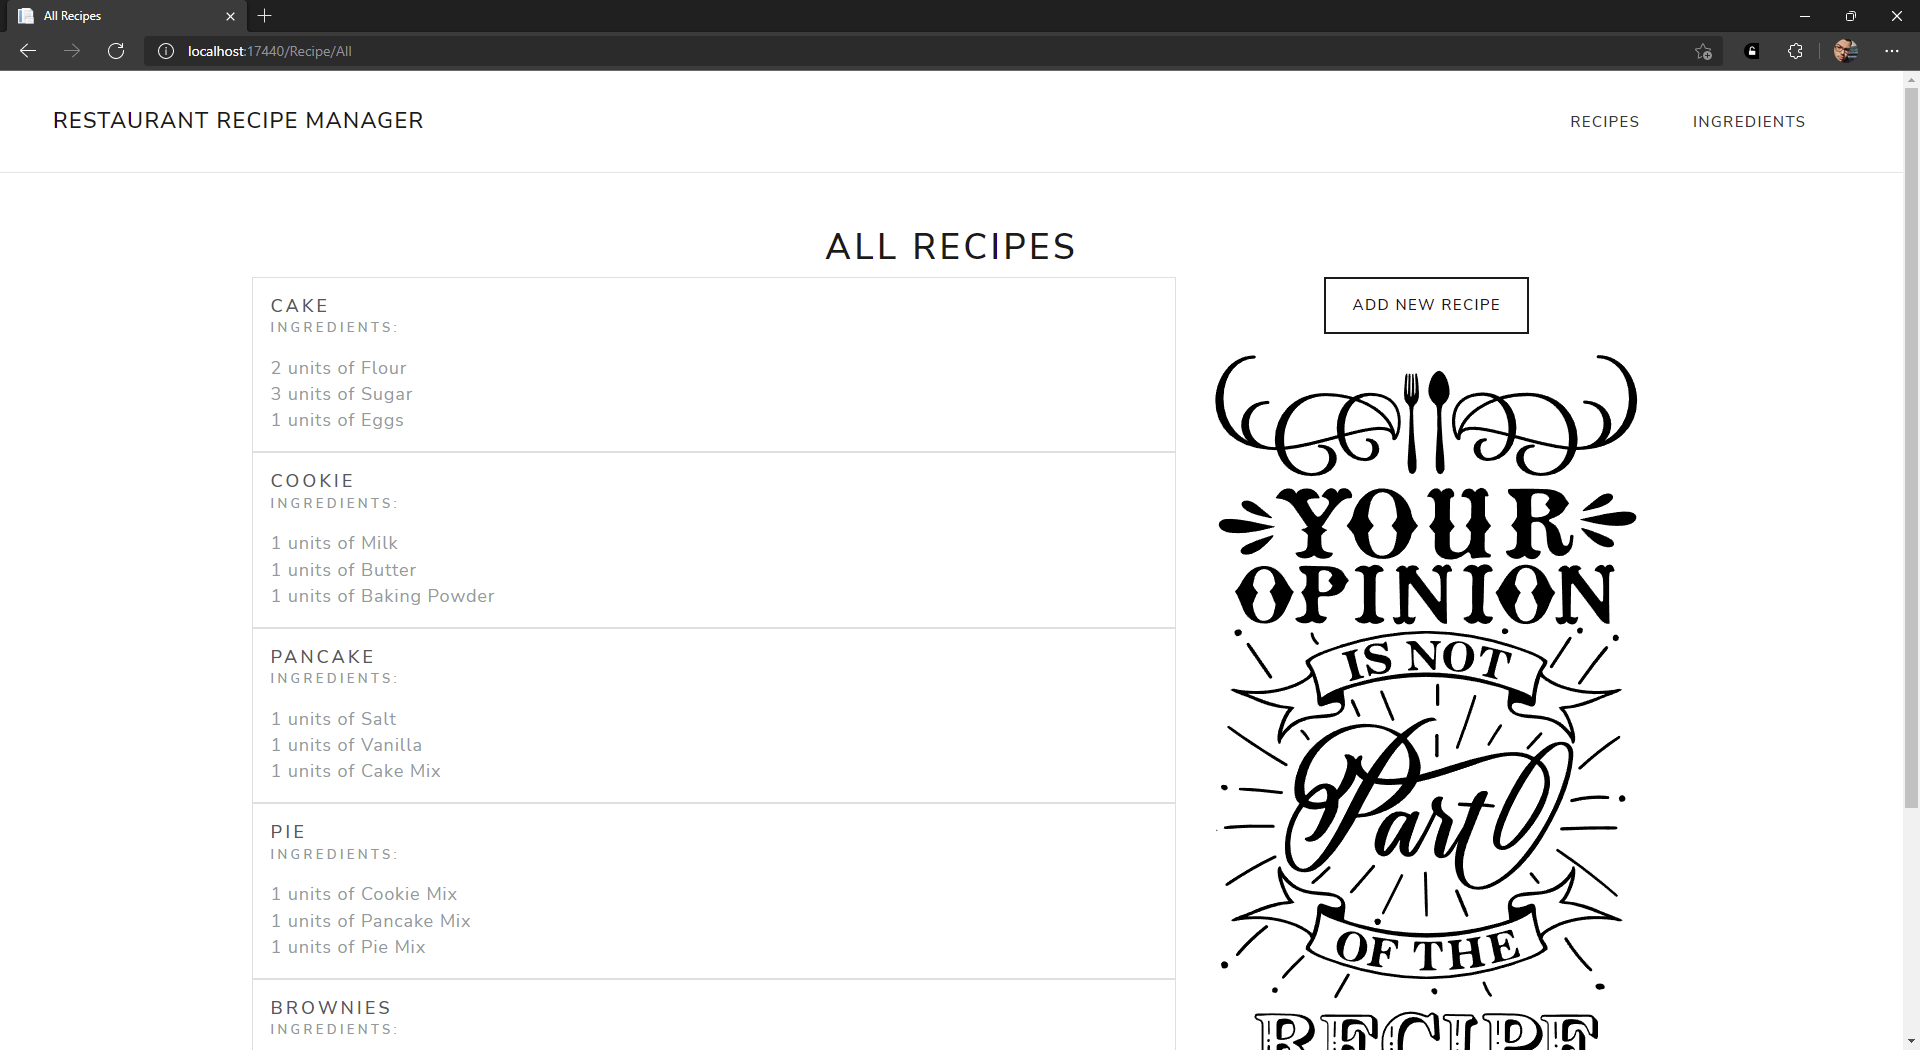
\includegraphics[width=14cm]{Resources/WebApp/Recipes/recipe (1).png}
    \caption{Ilustração da lista de Receitas}
    
\end{figure}
\FloatBarrier
\begin{figure}[!hbt]
    \centering
    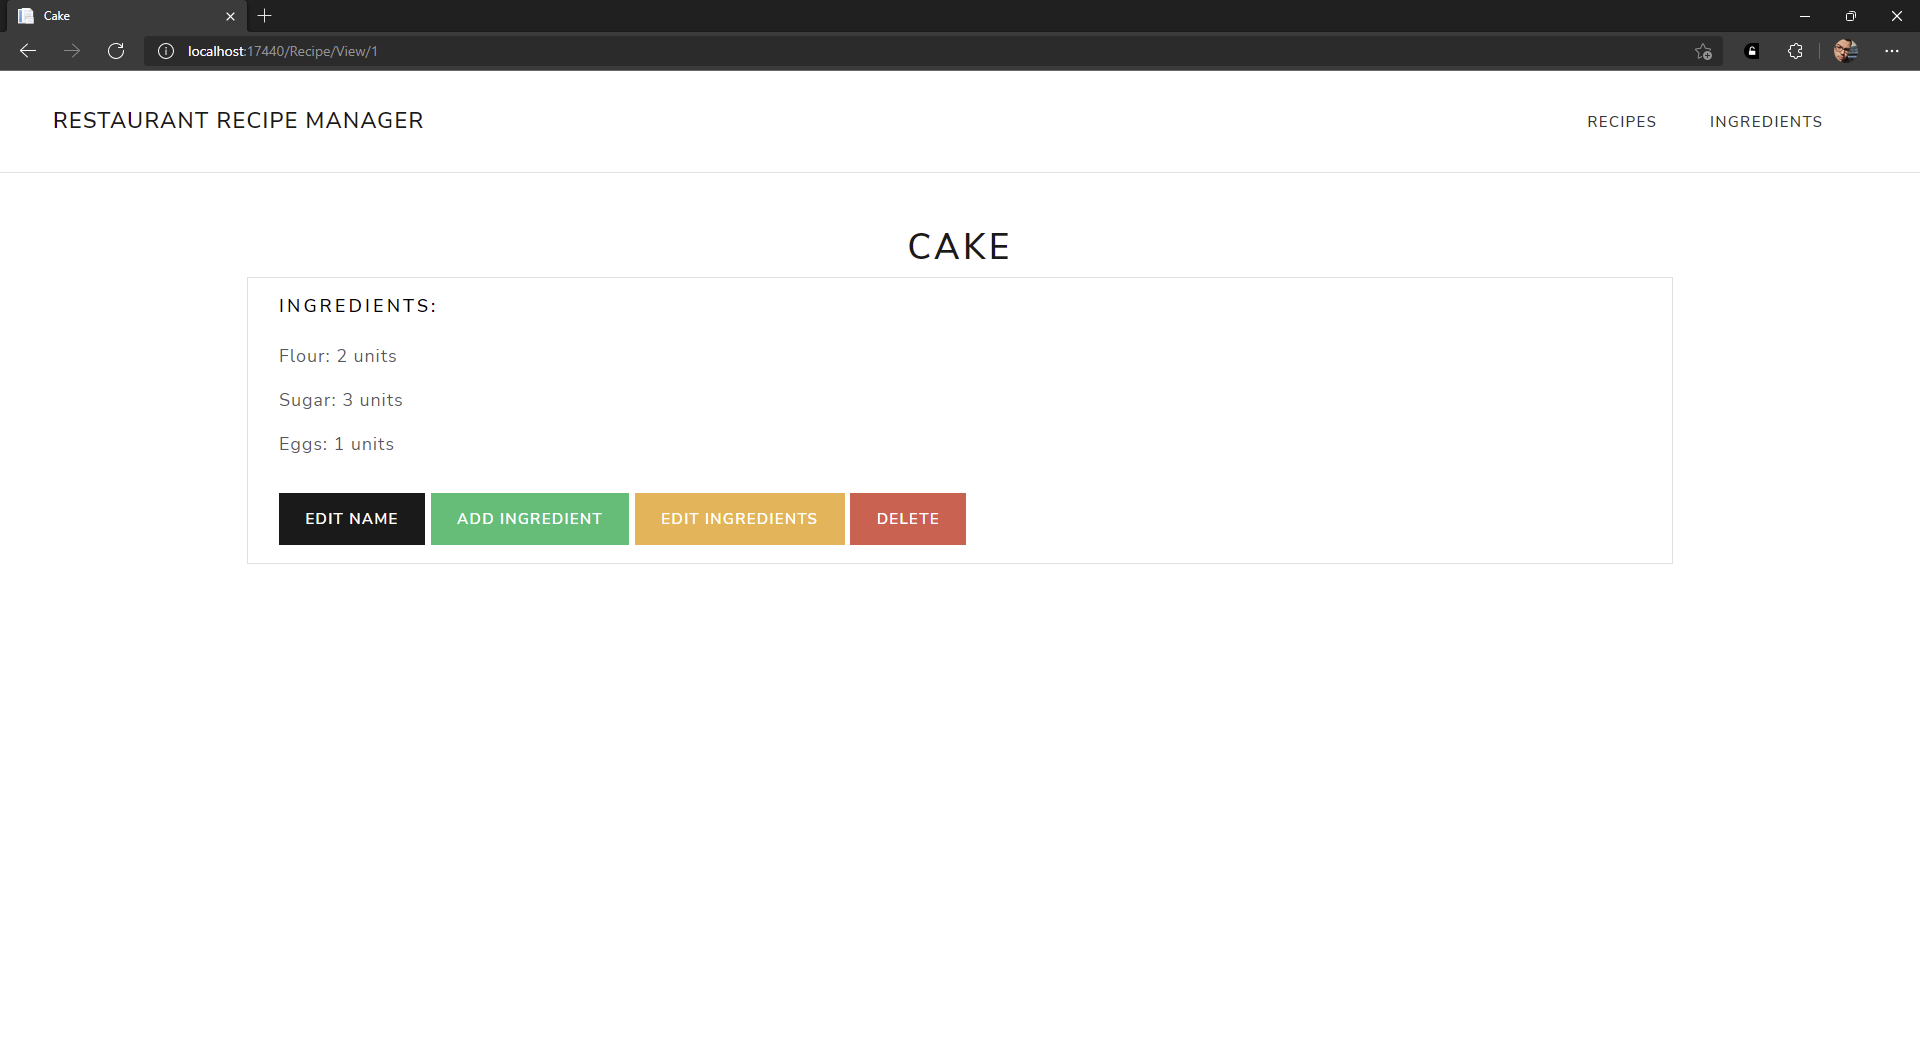
\includegraphics[width=14cm]{Resources/WebApp/Recipes/recipe (2).png}
    \caption{Ilustração da receita de Bolo}
    
\end{figure}
\FloatBarrier
\begin{figure}[!hbt]
    \centering
    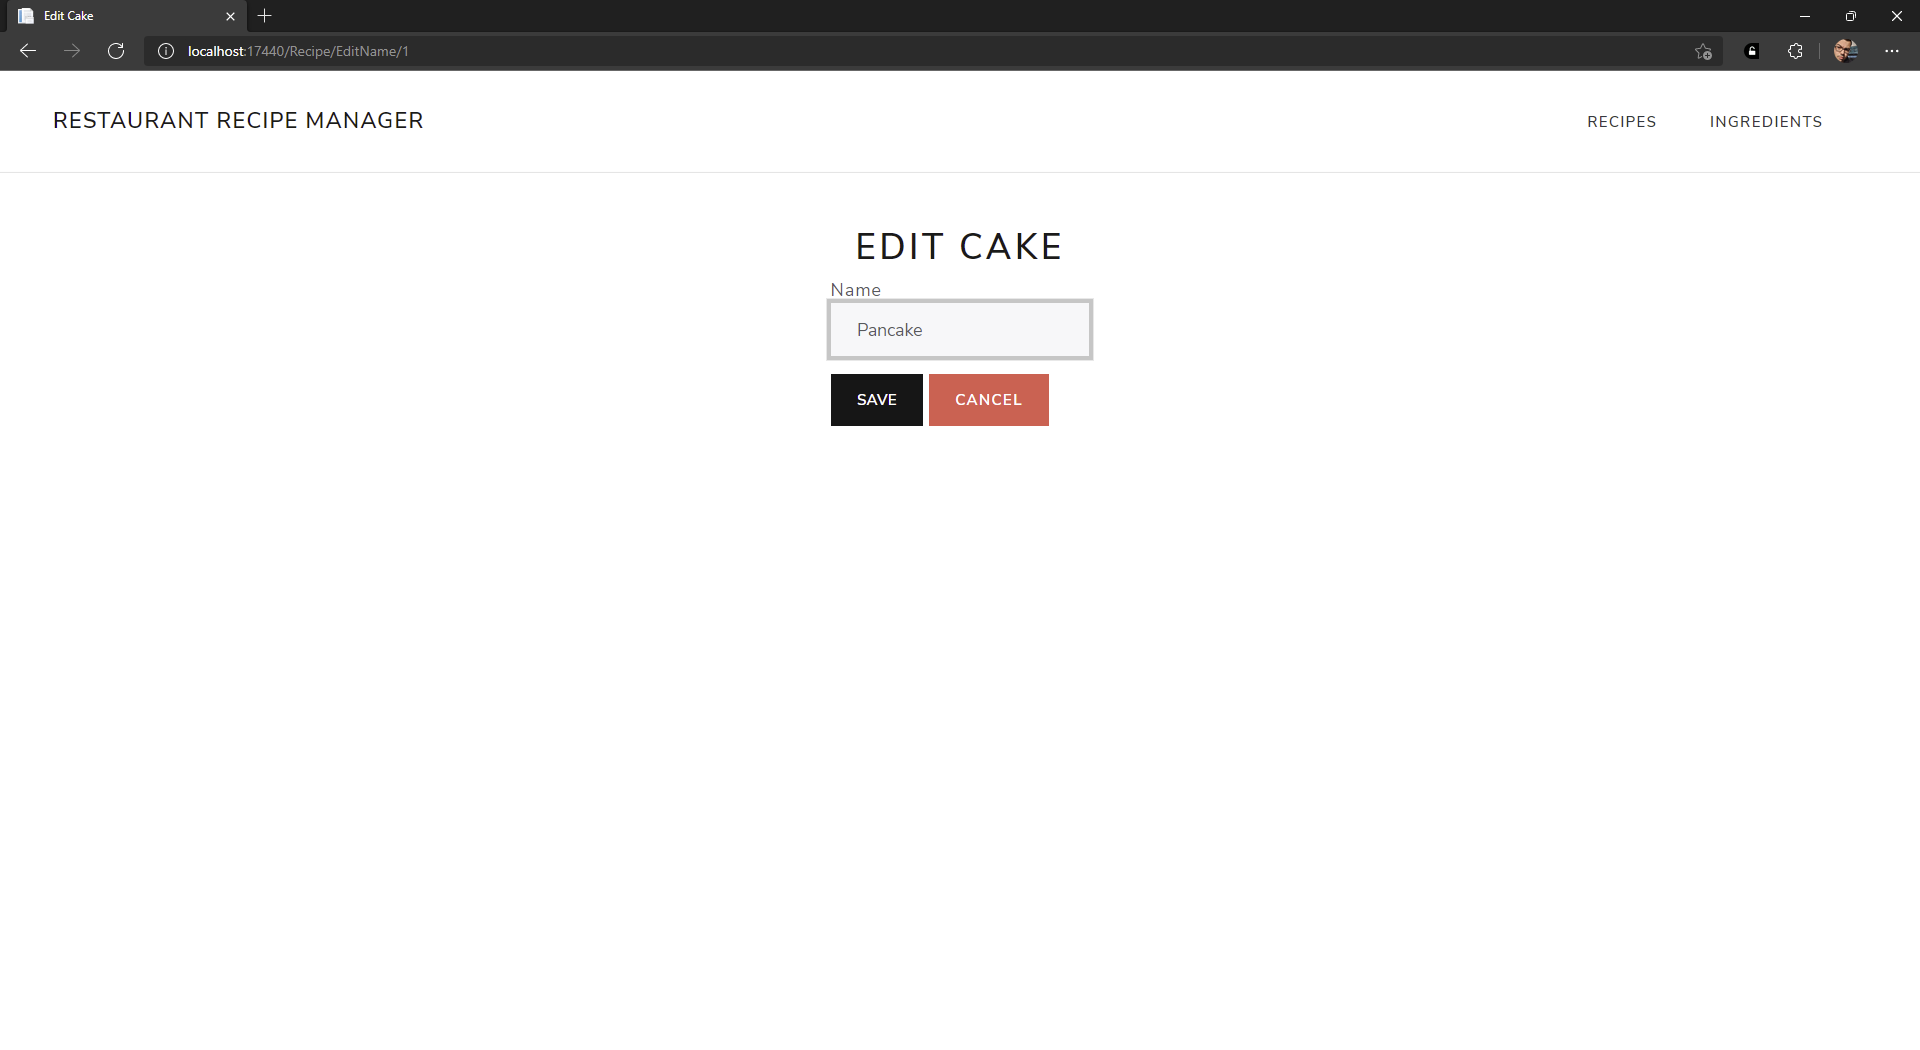
\includegraphics[width=14cm]{Resources/WebApp/Recipes/recipe (3).png}
    \caption{Ilustração dedição da receita de Bolo}
    
\end{figure}
\FloatBarrier
\begin{figure}[!hbt]
    \centering
    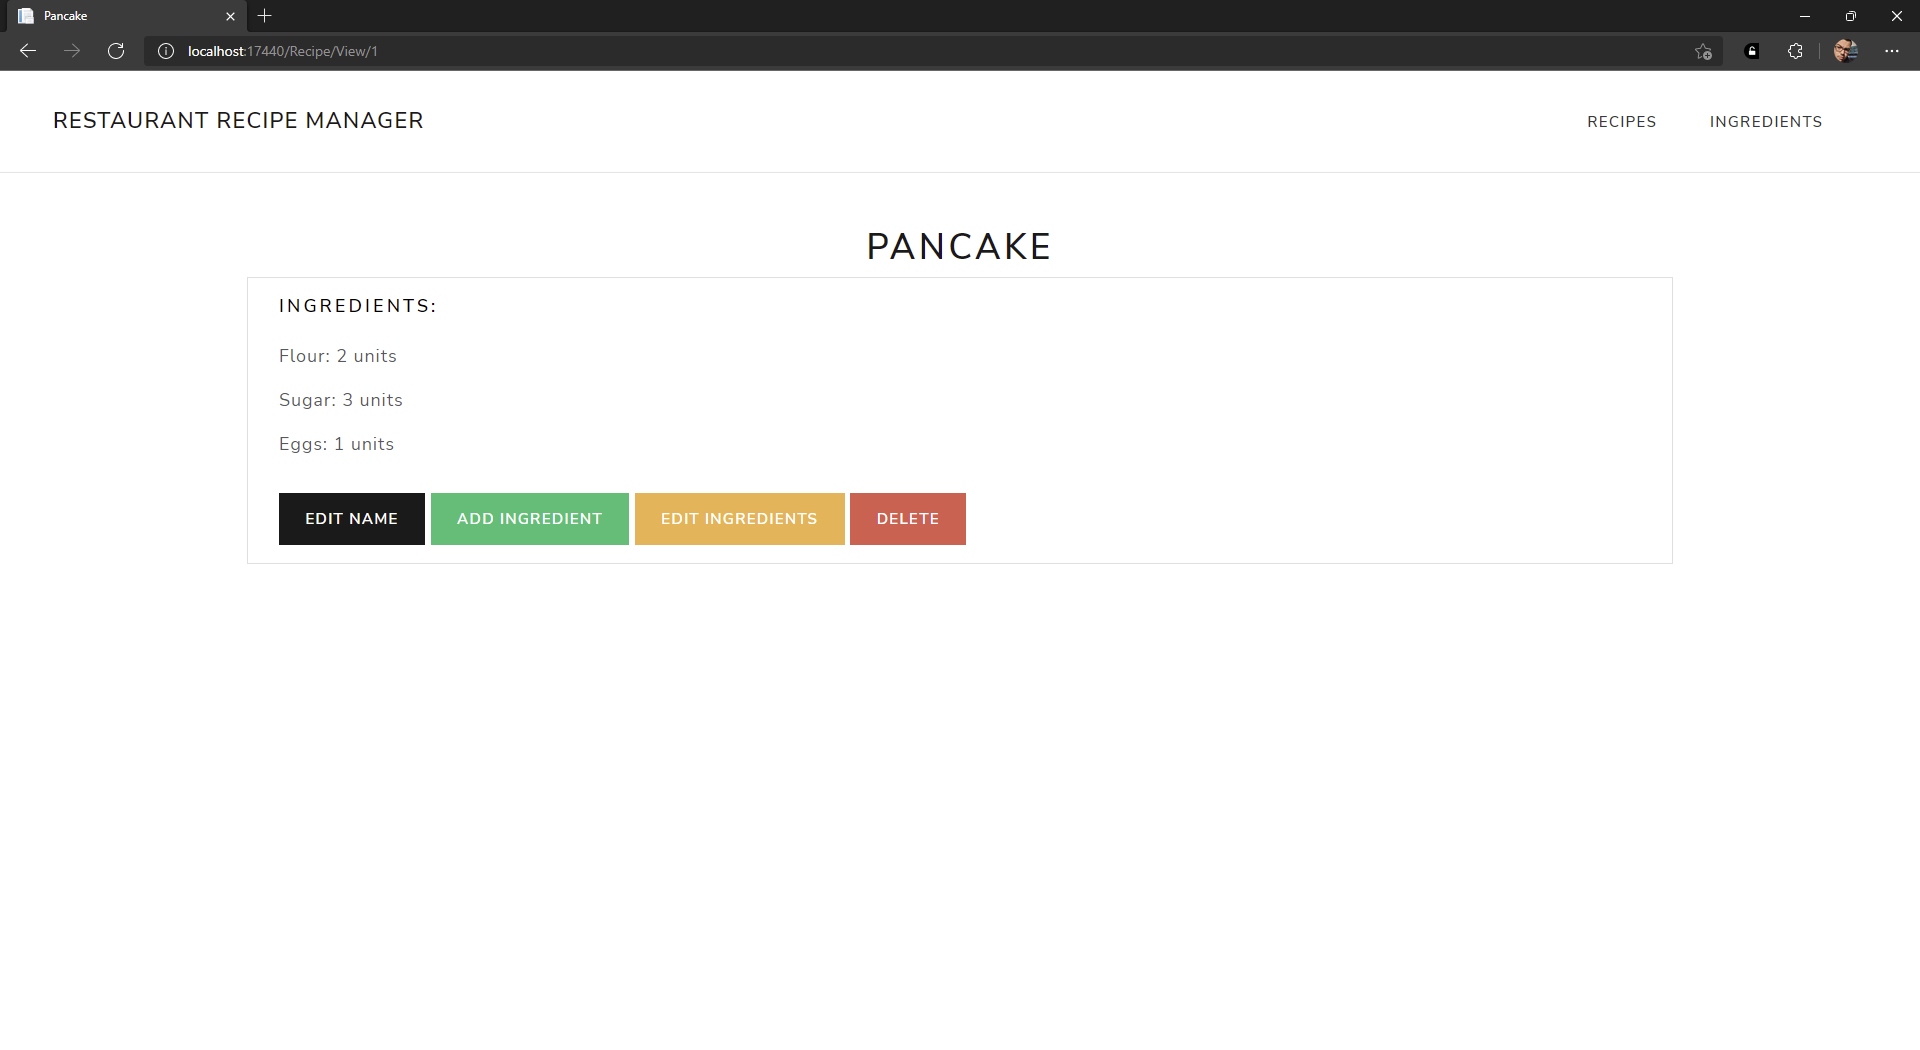
\includegraphics[width=14cm]{Resources/WebApp/Recipes/recipe (4).png}
    \caption{Ilustração da receita renomeada para Panqueca}
    
\end{figure}
\FloatBarrier
\begin{figure}[!hbt]
    \centering
    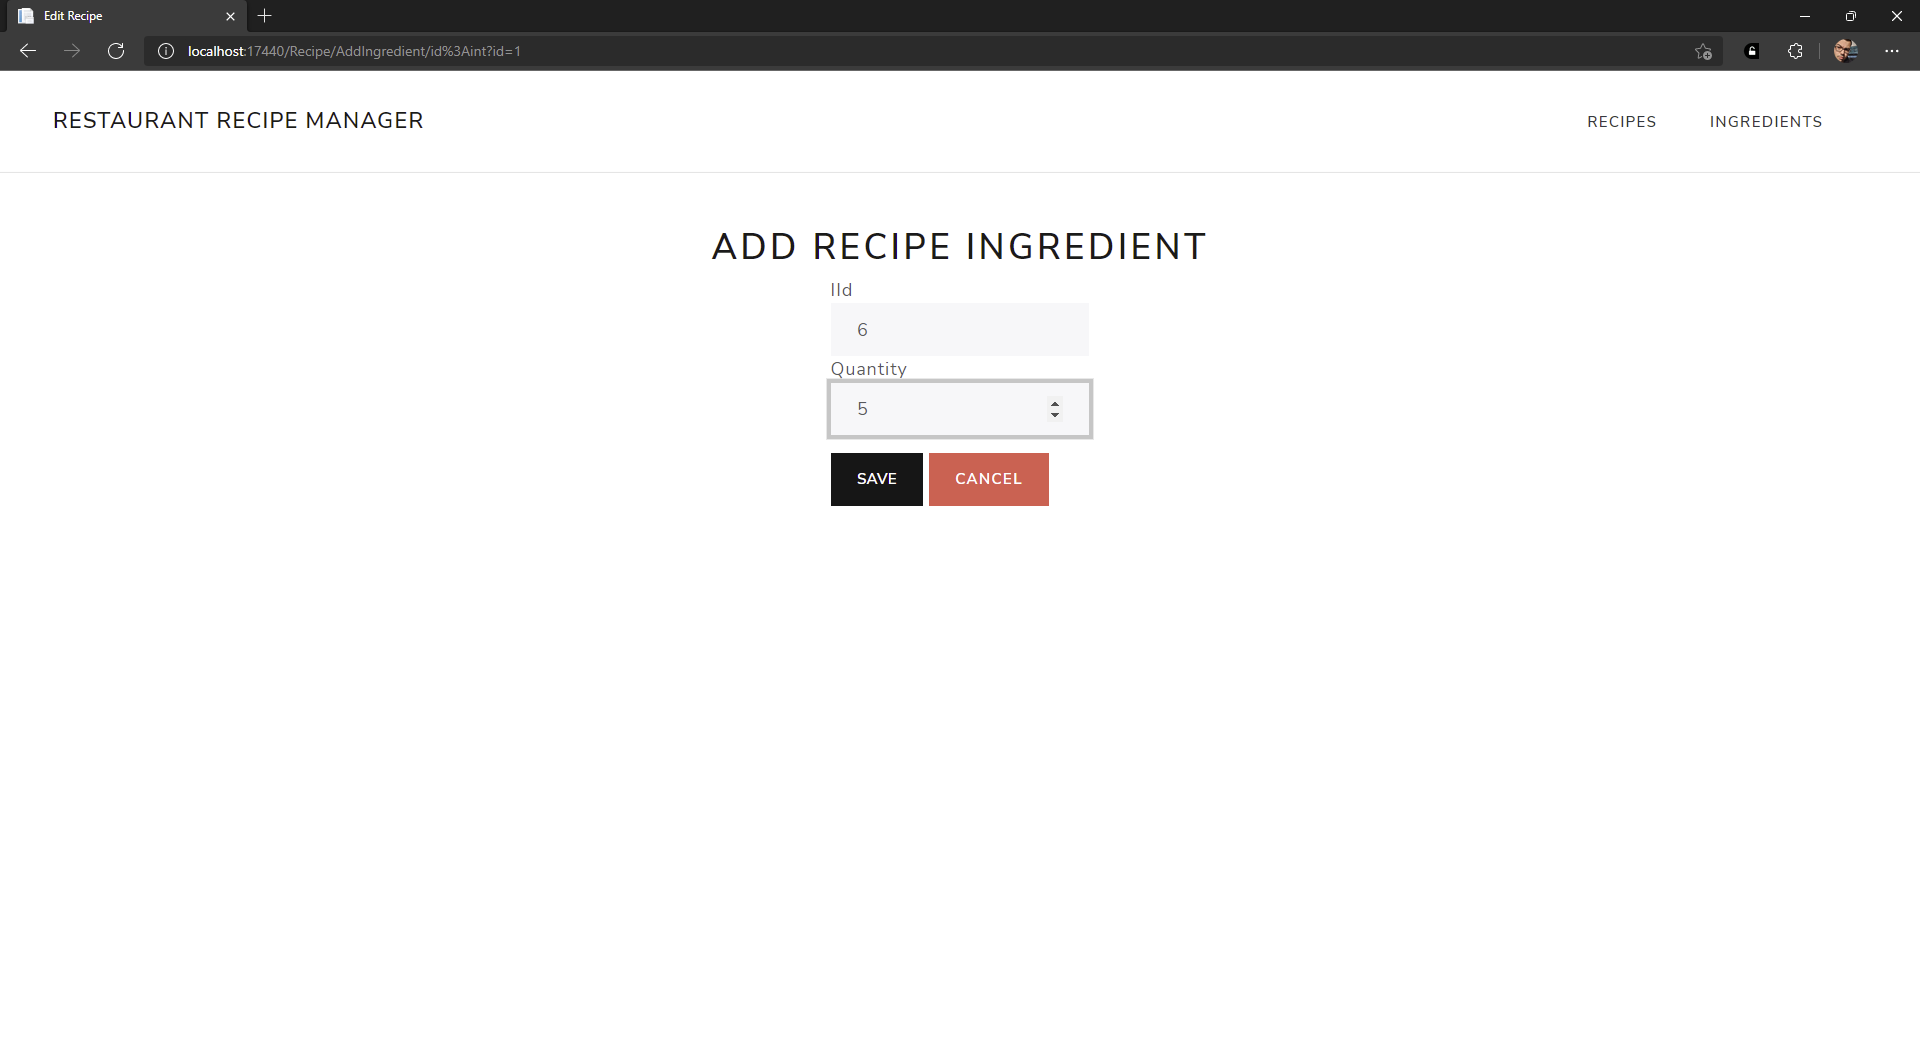
\includegraphics[width=14cm]{Resources/WebApp/Recipes/recipe (5).png}
    \caption{Ilustração da adição de Fermento à receita}
    
\end{figure}
\FloatBarrier
\begin{figure}[!hbt]
    \centering
    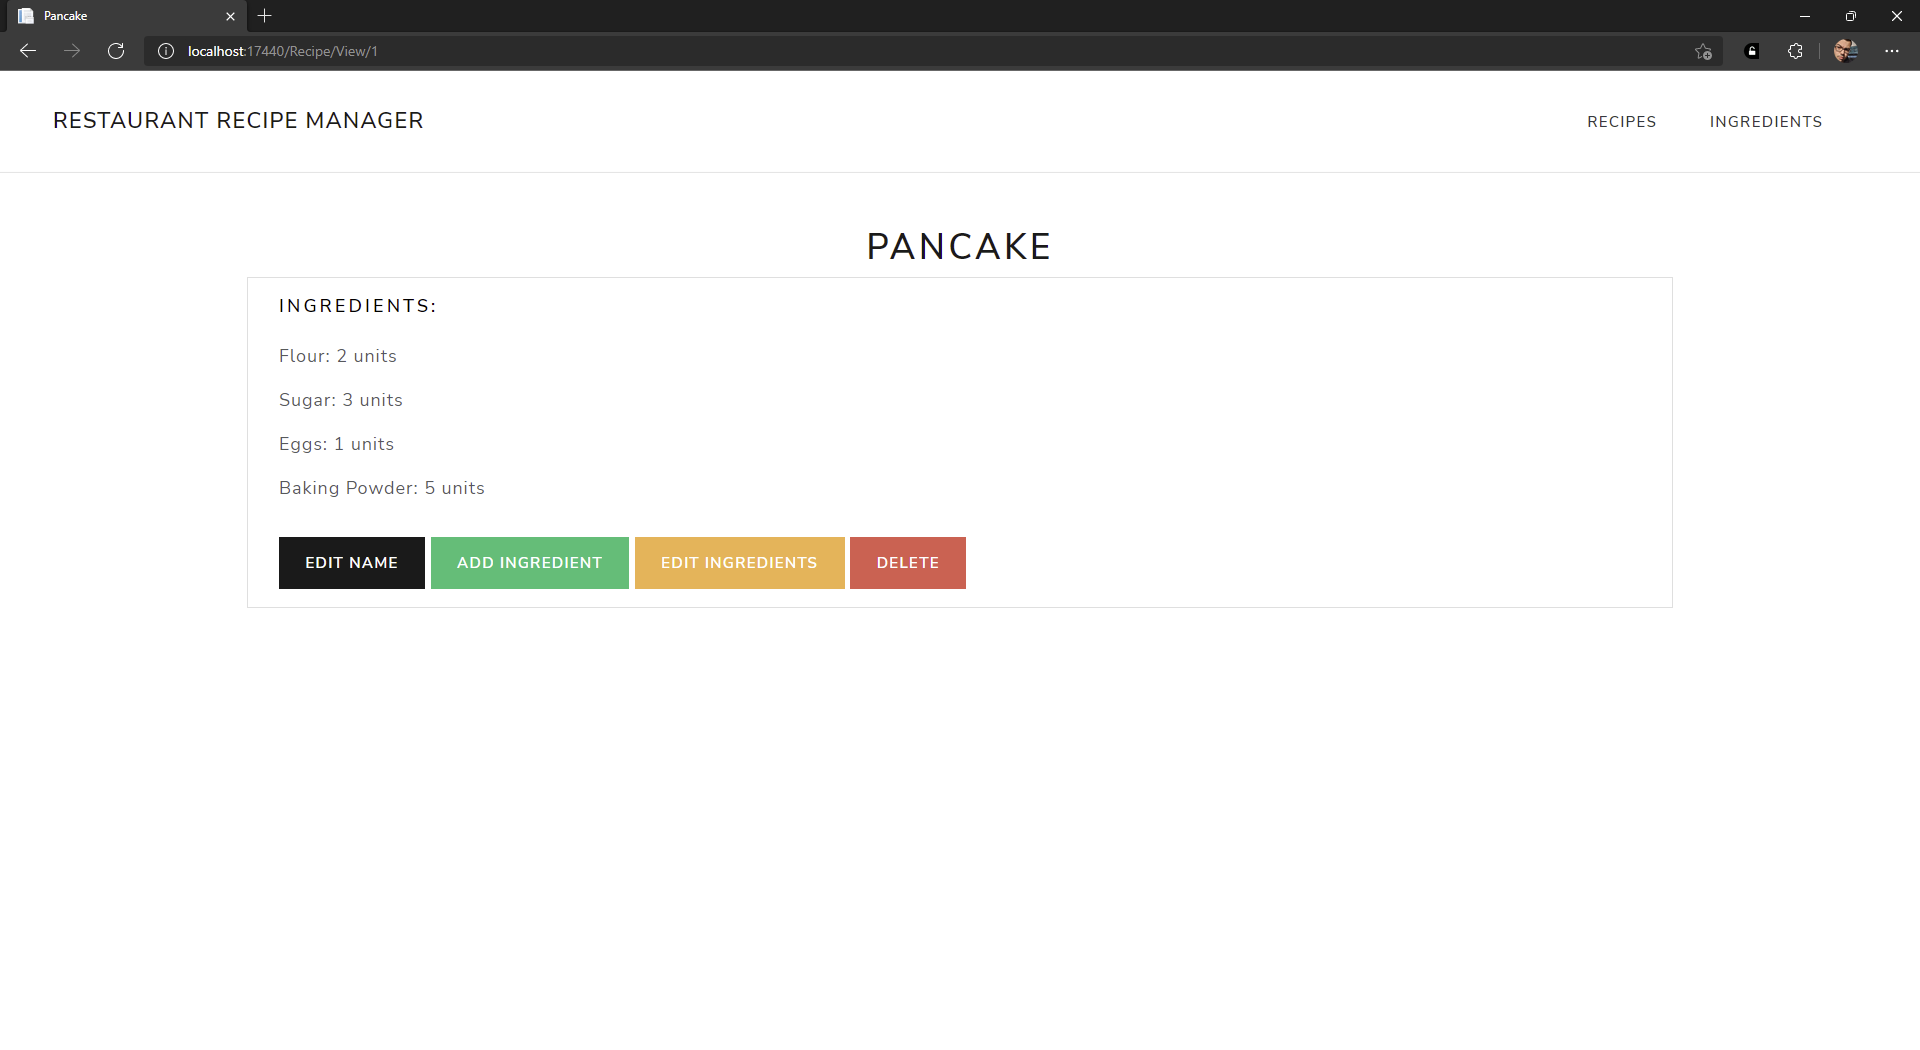
\includegraphics[width=14cm]{Resources/WebApp/Recipes/recipe (6).png}
    \caption{Ilustração da receita com Fermento adicionado}
    
\end{figure}
\FloatBarrier
\begin{figure}[!hbt]
    \centering
    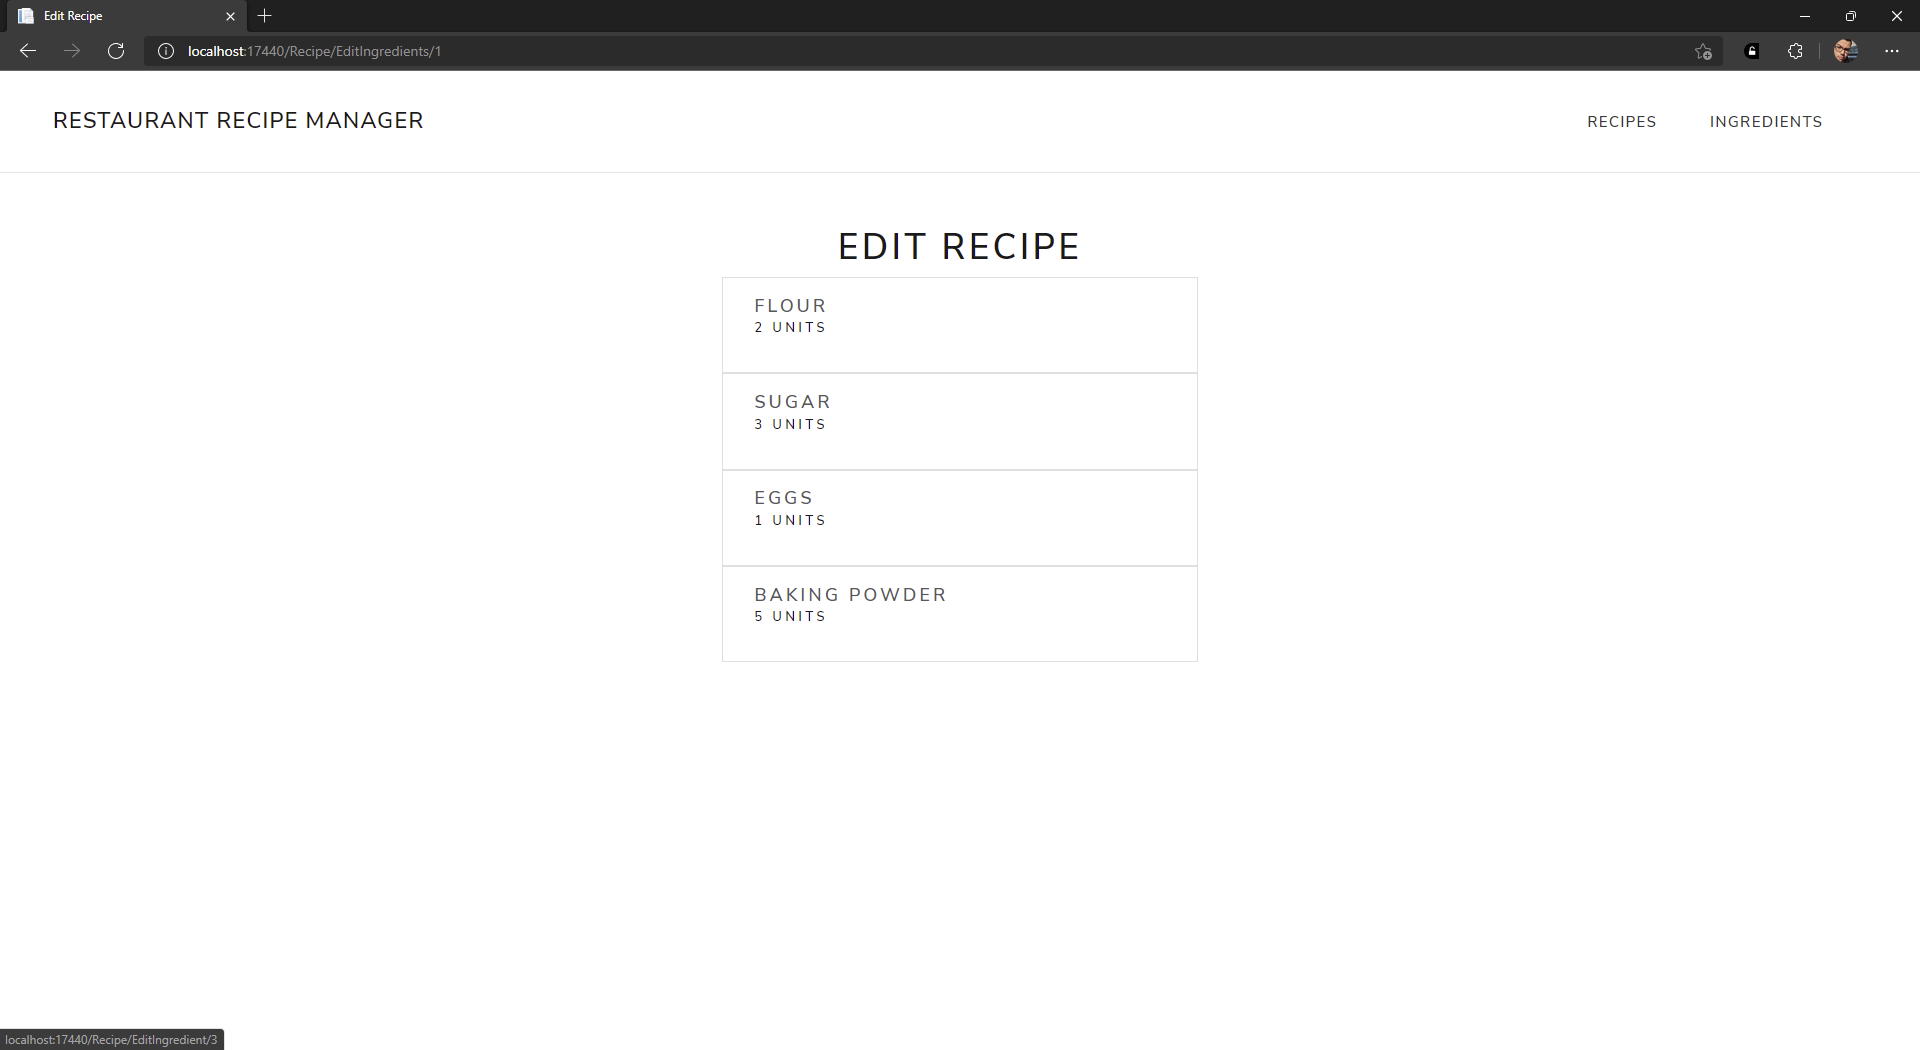
\includegraphics[width=14cm]{Resources/WebApp/Recipes/recipe (7).png}
    \caption{Ilustração da lista de ingredientes da Panqueca para alterar}
    
\end{figure}
\FloatBarrier
\begin{figure}[!hbt]
    \centering
    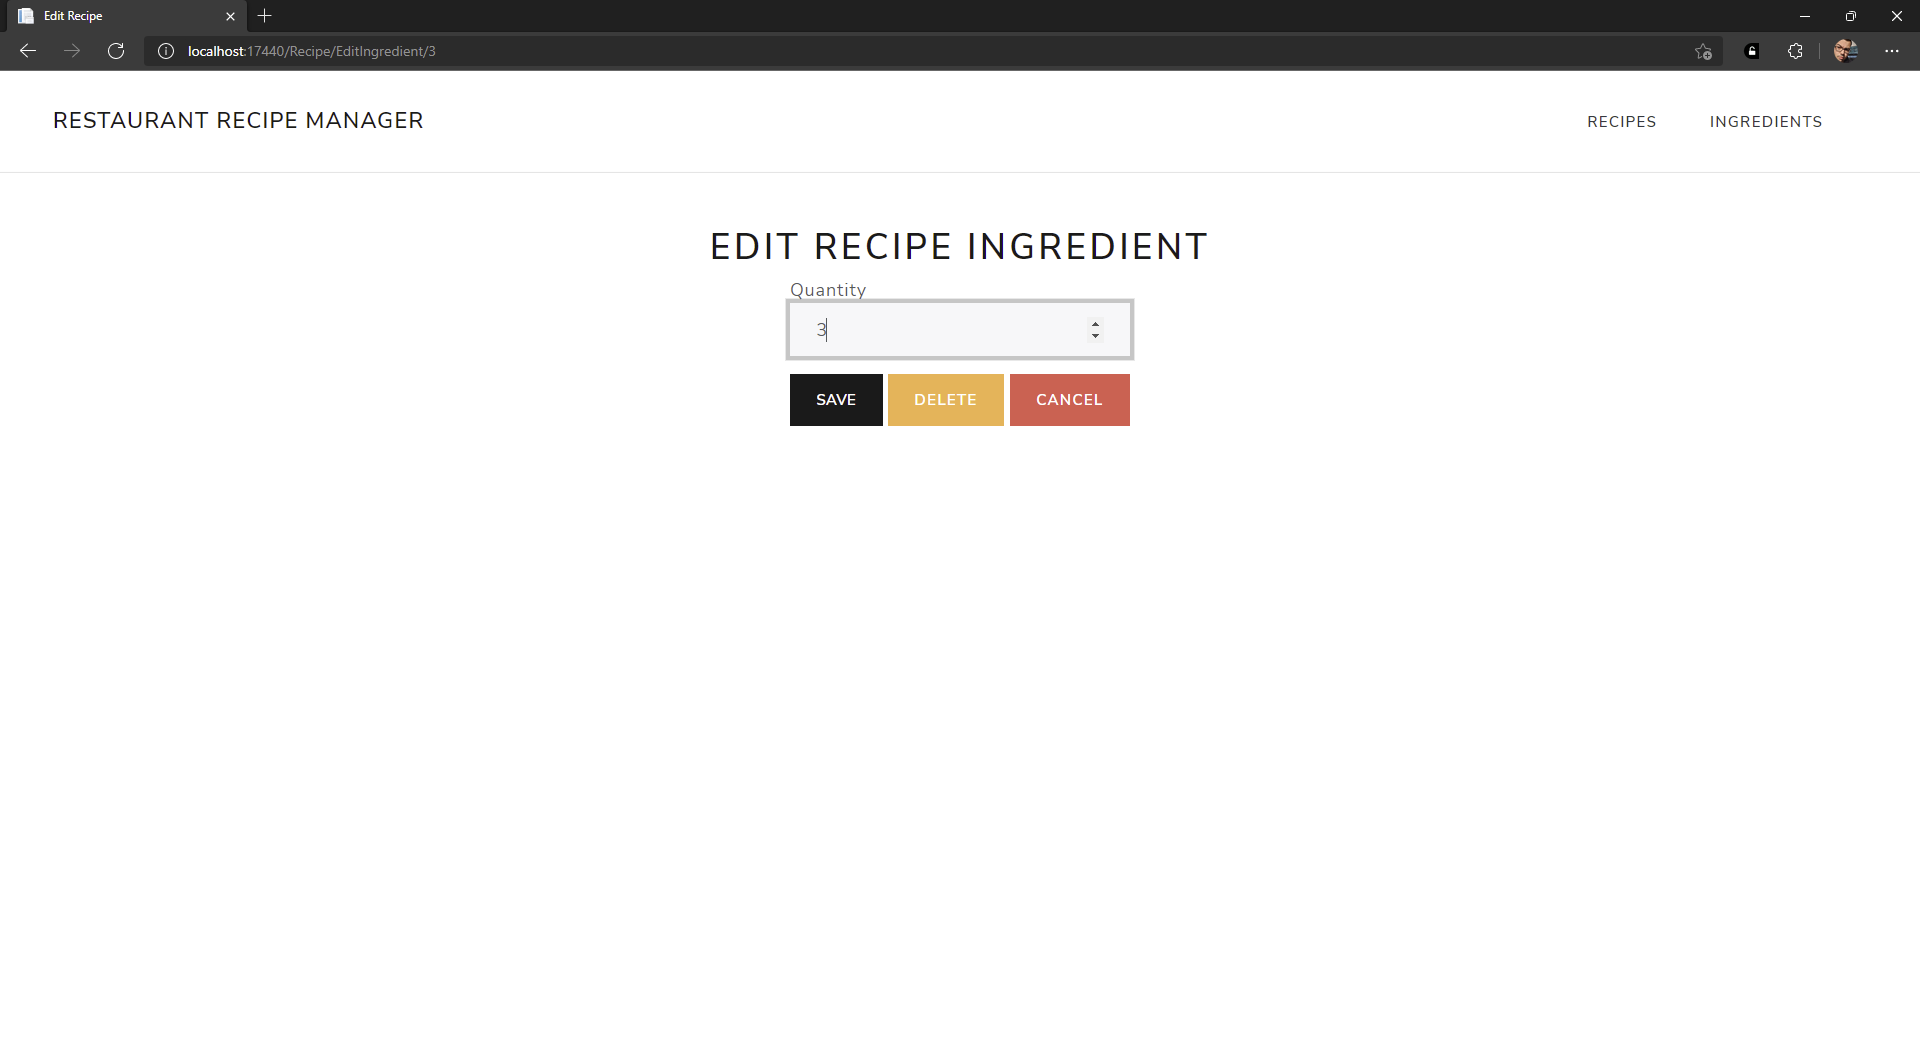
\includegraphics[width=14cm]{Resources/WebApp/Recipes/recipe (8).png}
    \caption{Ilustração do edição da quantidade ou eliminação de um ingrediente}
    
\end{figure}
\FloatBarrier
\begin{figure}[!hbt]
    \centering
    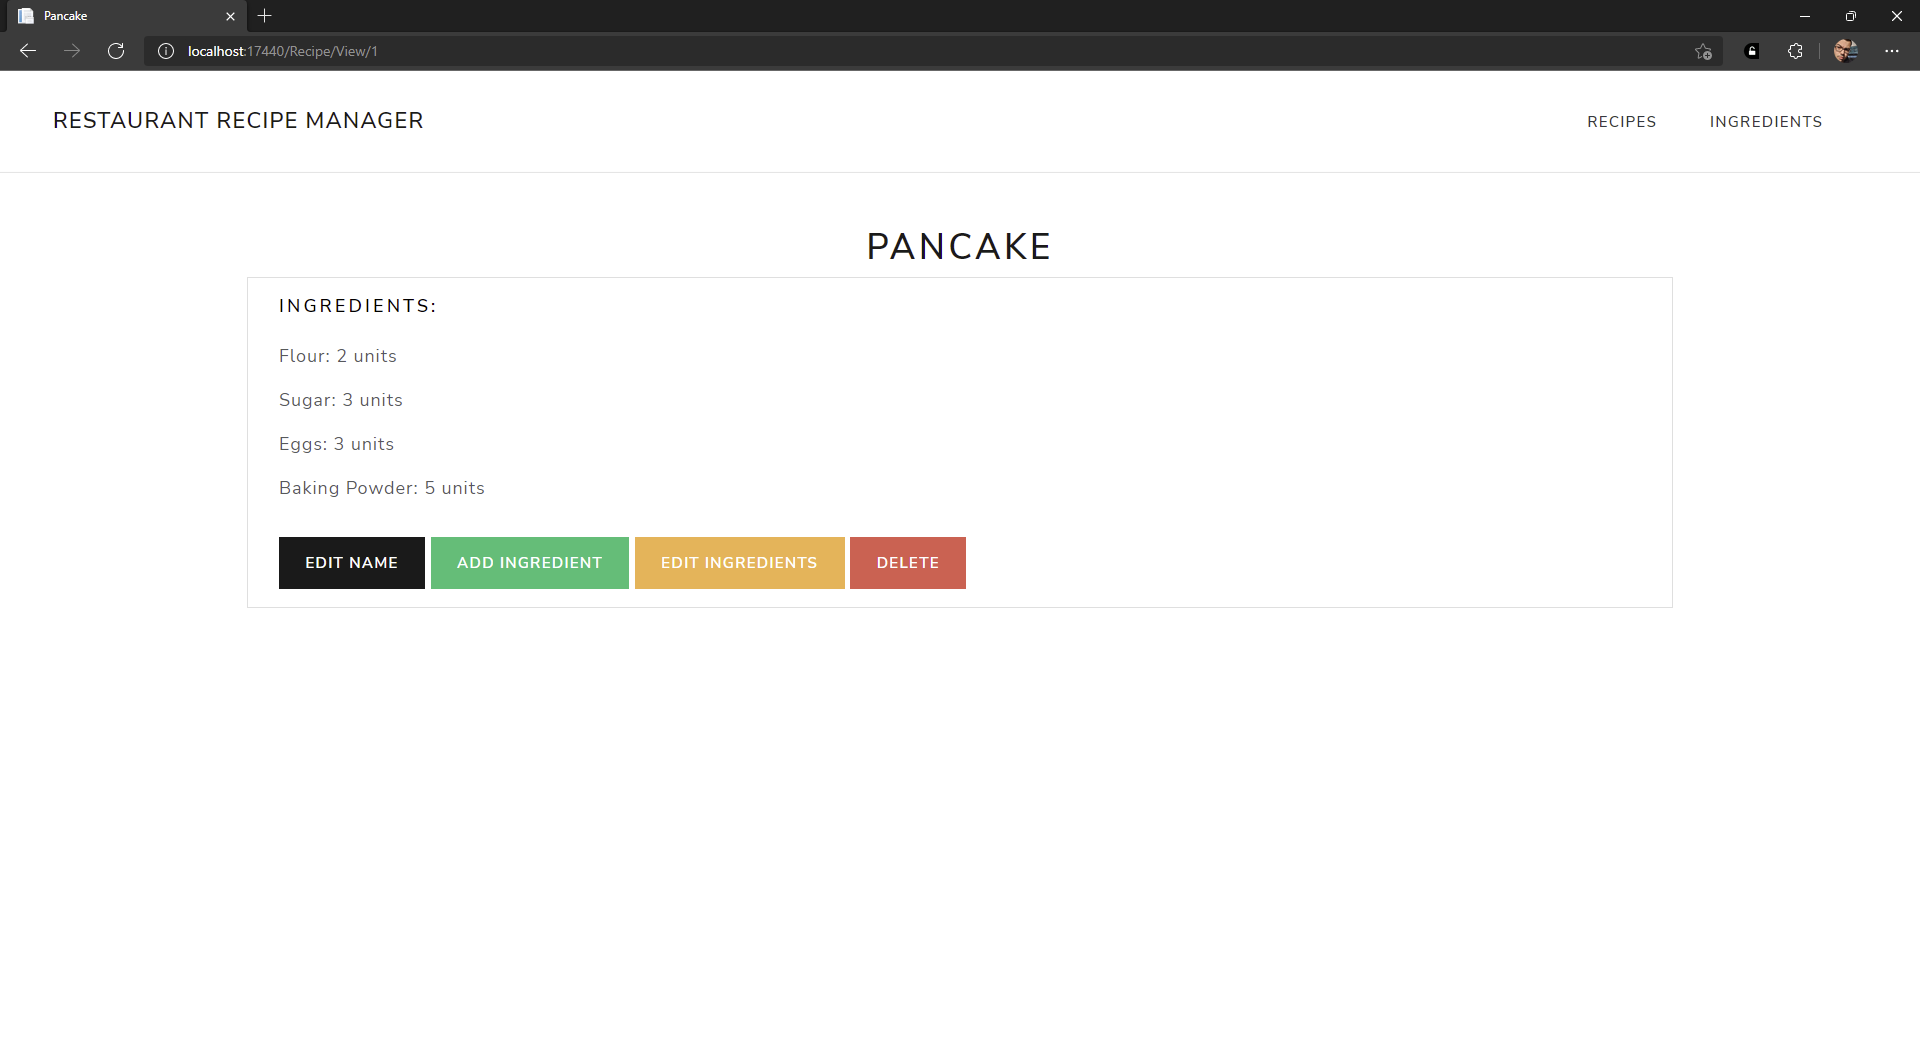
\includegraphics[width=14cm]{Resources/WebApp/Recipes/recipe (9).png}
    \caption{Ilustração da lista de Receitas com a Panqueca sem o ingrediente removido}
    
\end{figure}
\FloatBarrier
\begin{figure}[!hbt]
    \centering
    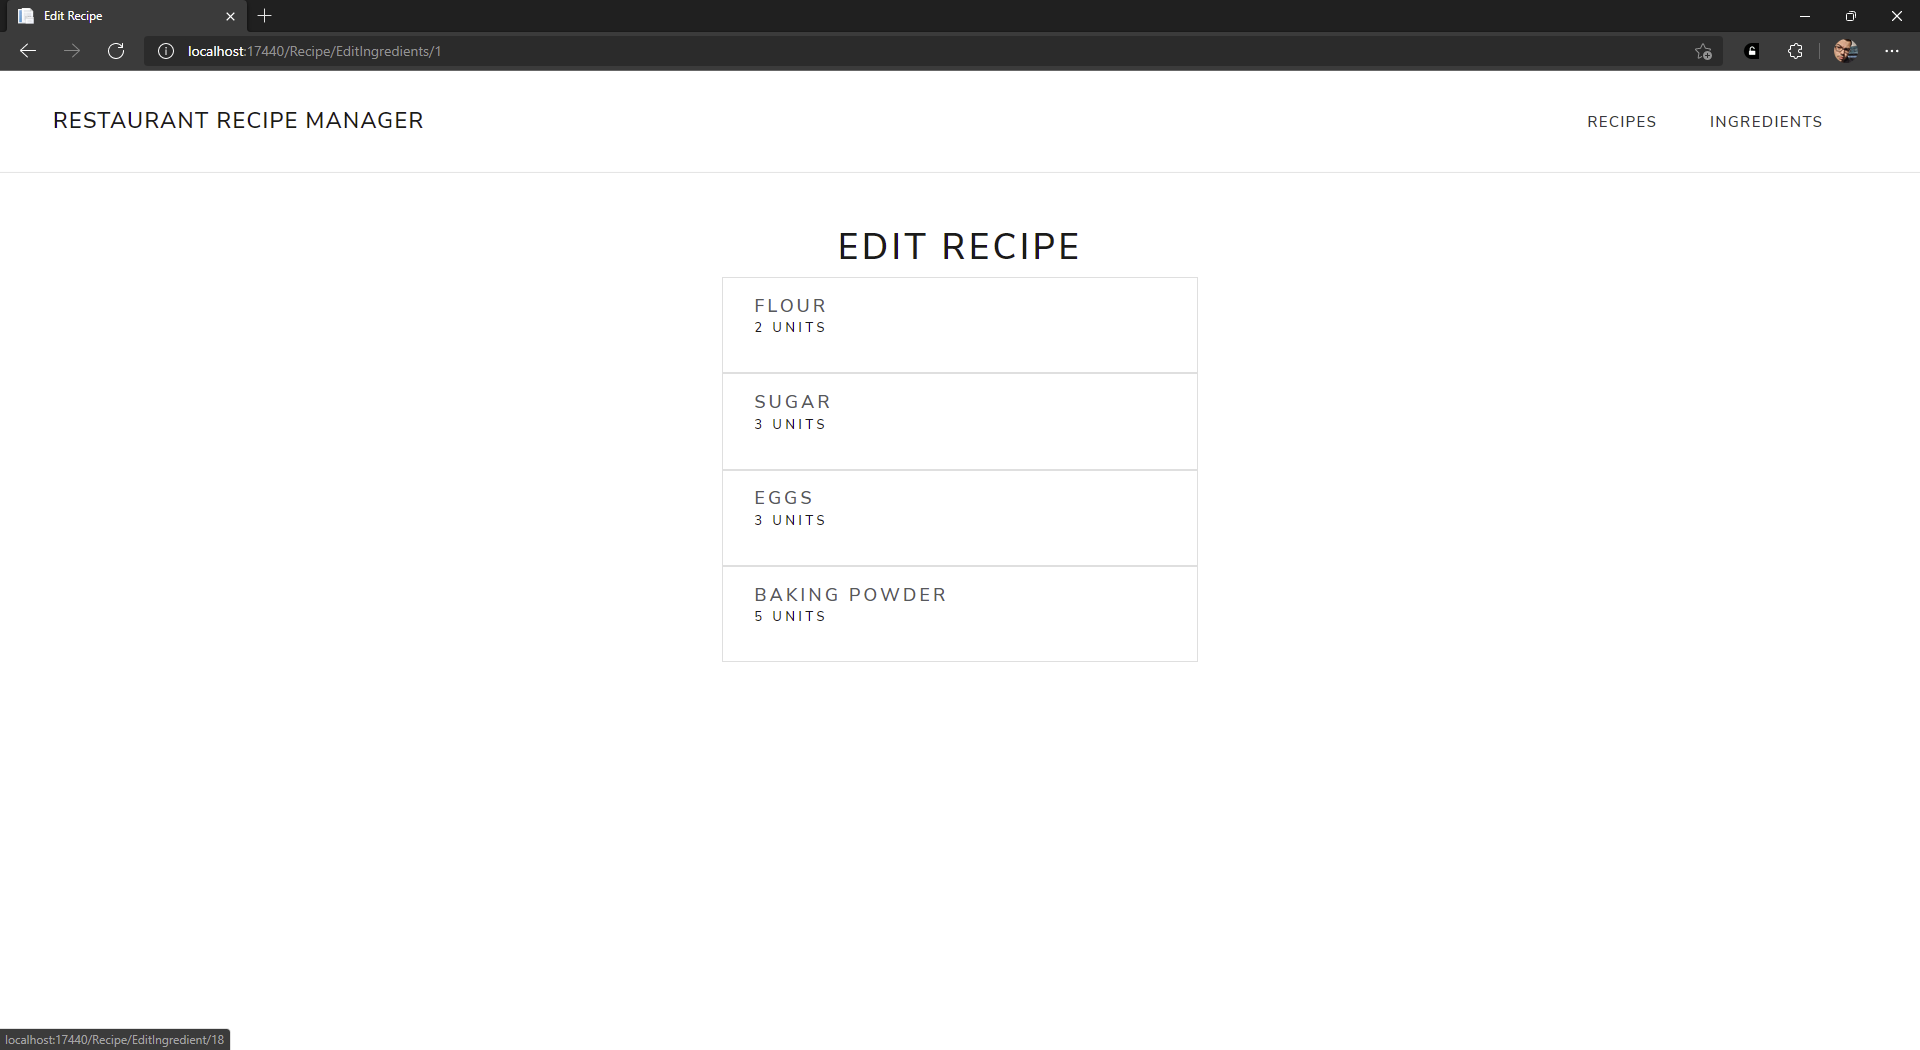
\includegraphics[width=14cm]{Resources/WebApp/Recipes/recipe (10).png}
    \caption{Ilustração da edição de uma Receita, com os ingredientes listados}
    
\end{figure}
\FloatBarrier
\begin{figure}[!hbt]
    \centering
    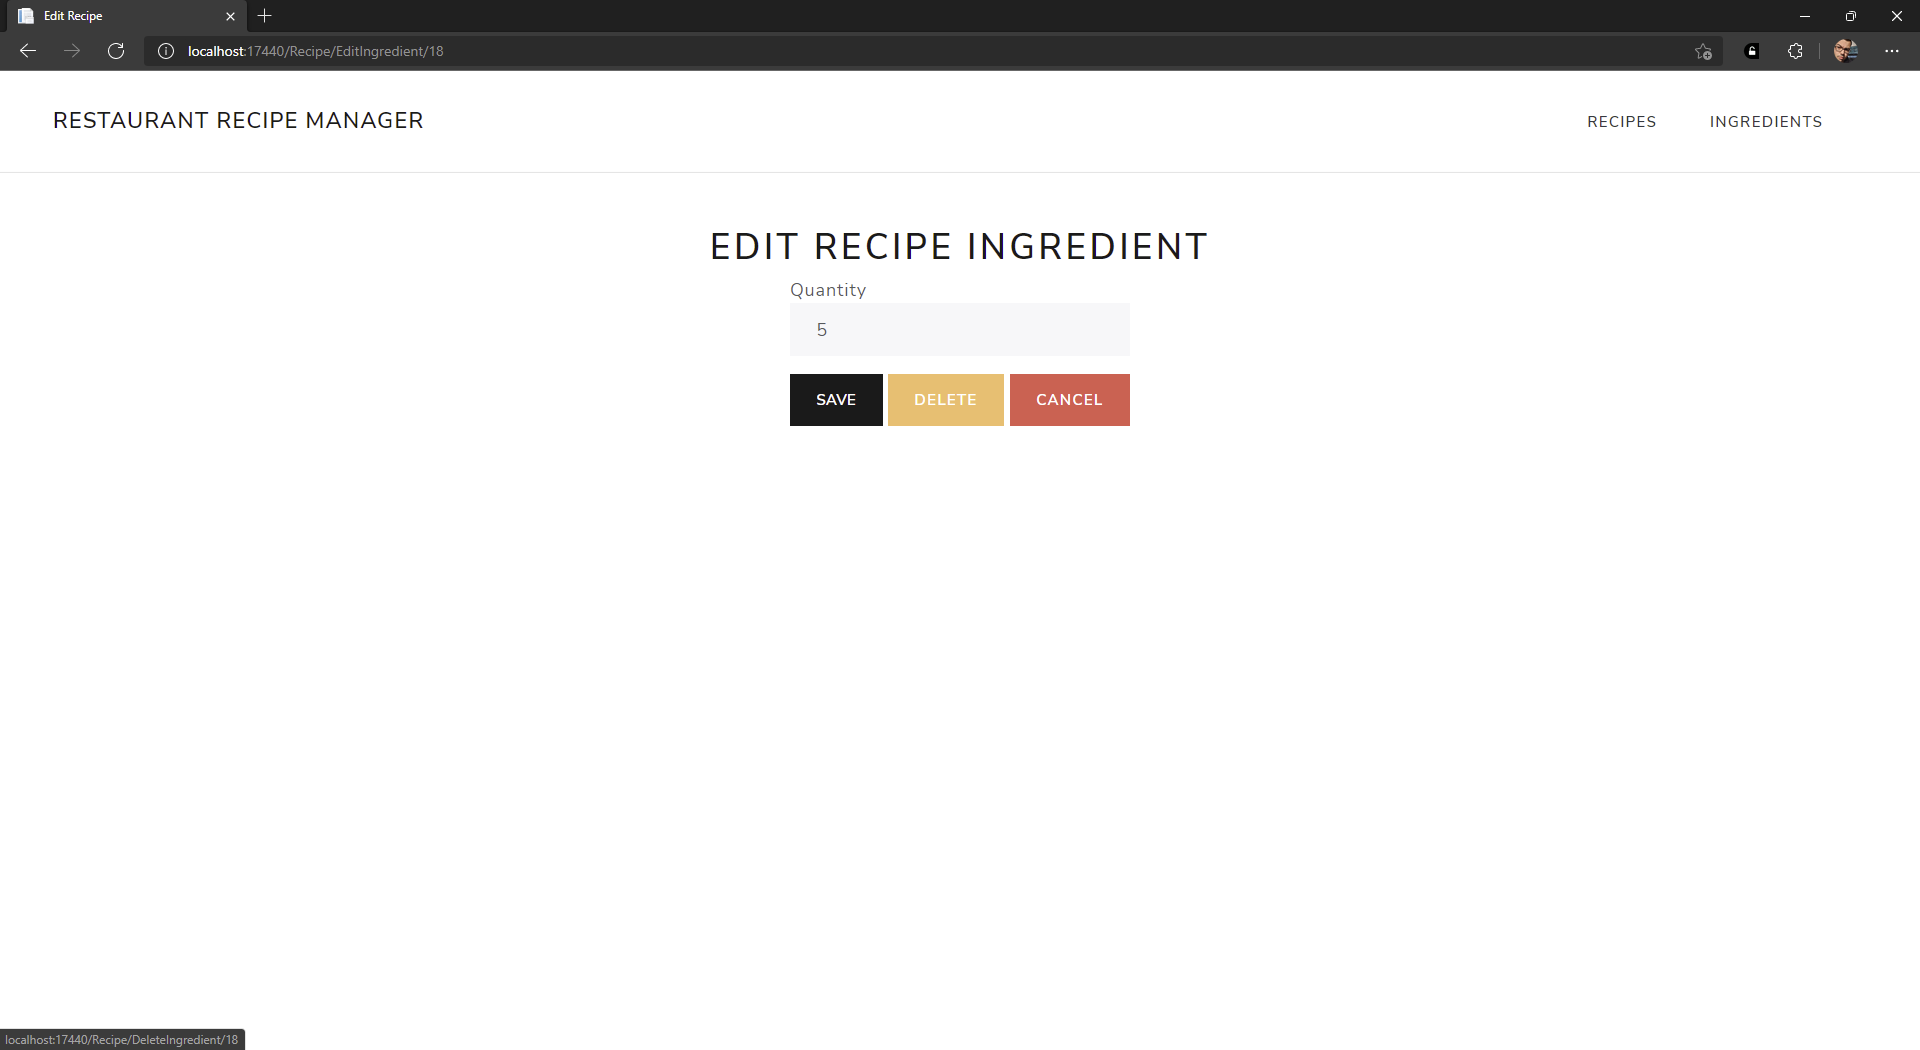
\includegraphics[width=14cm]{Resources/WebApp/Recipes/recipe (11).png}
    \caption{Ilustração da eliminação do Fermento}
    
\end{figure}
\FloatBarrier
\begin{figure}[!hbt]
    \centering
    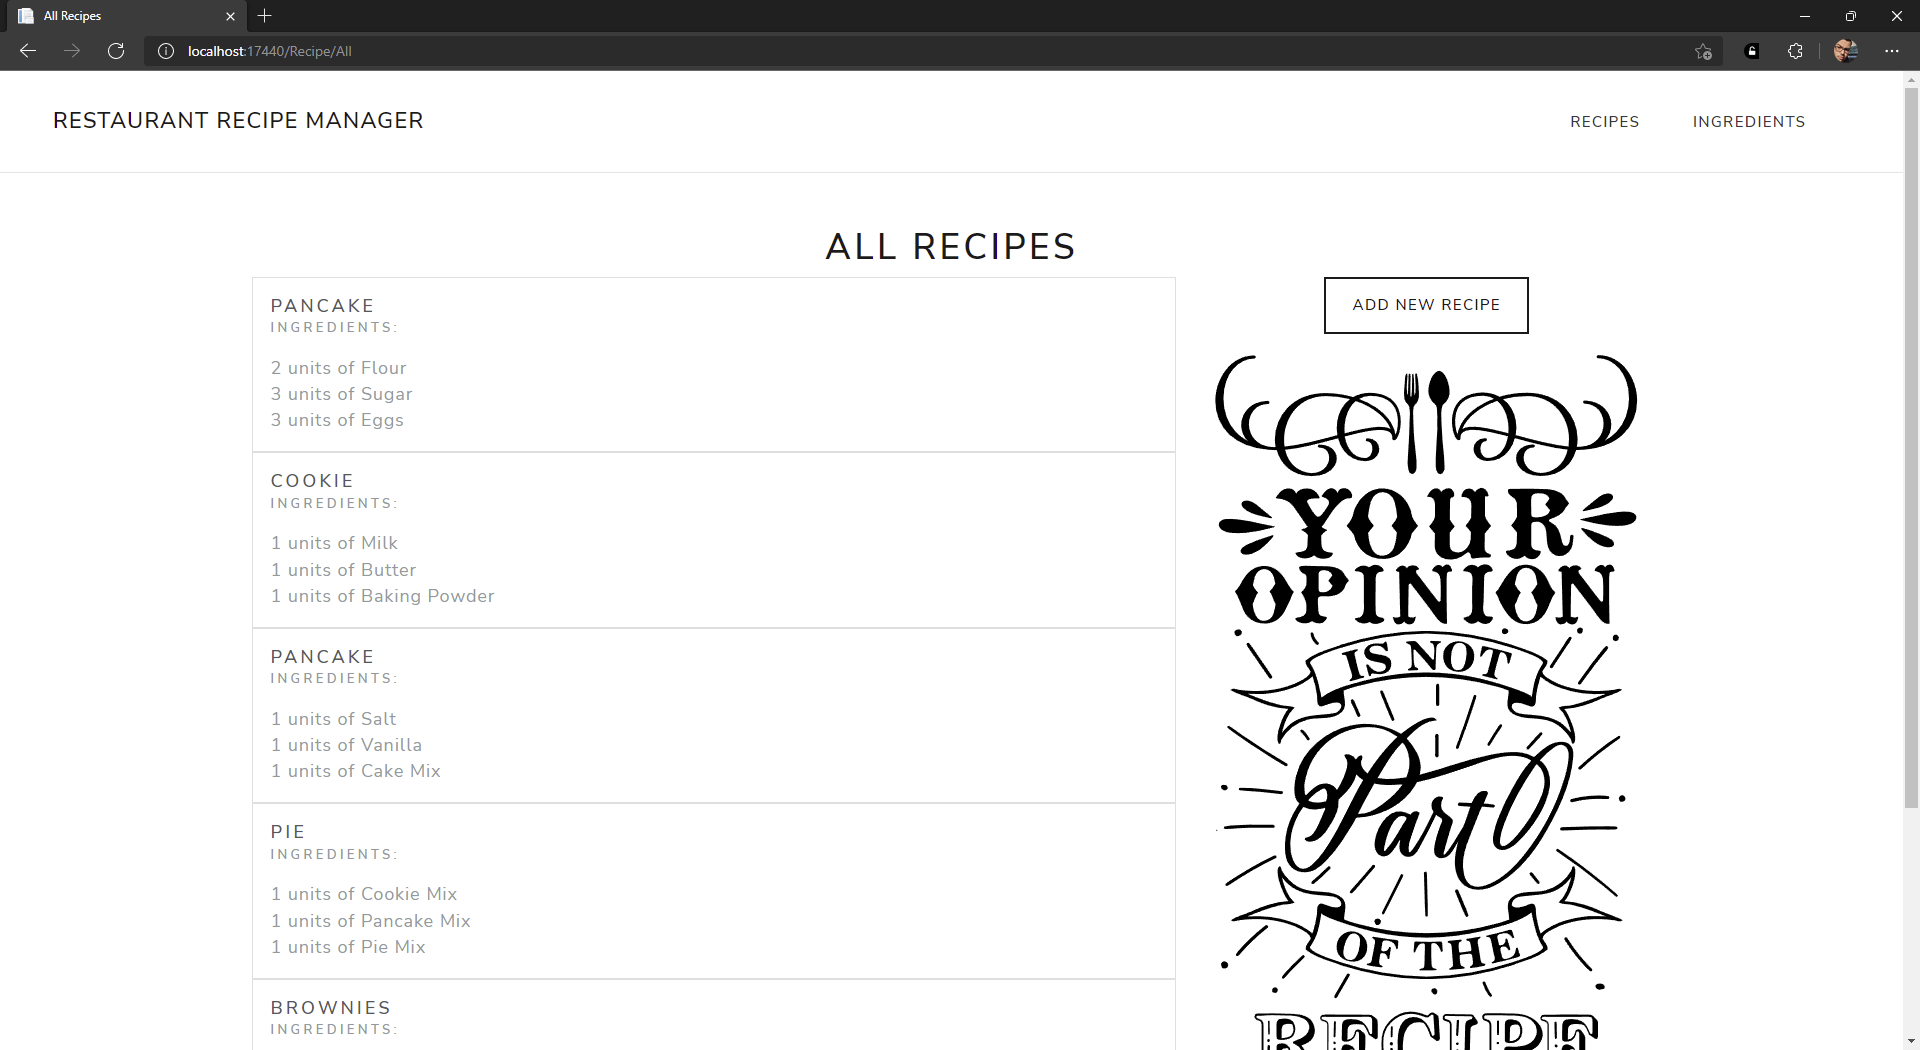
\includegraphics[width=14cm]{Resources/WebApp/Recipes/recipe (12).png}
    \caption{Ilustração da lista de Receitas sem o Fermento na Panqueca}
    
\end{figure}
\FloatBarrier
\begin{figure}[!hbt]
    \centering
    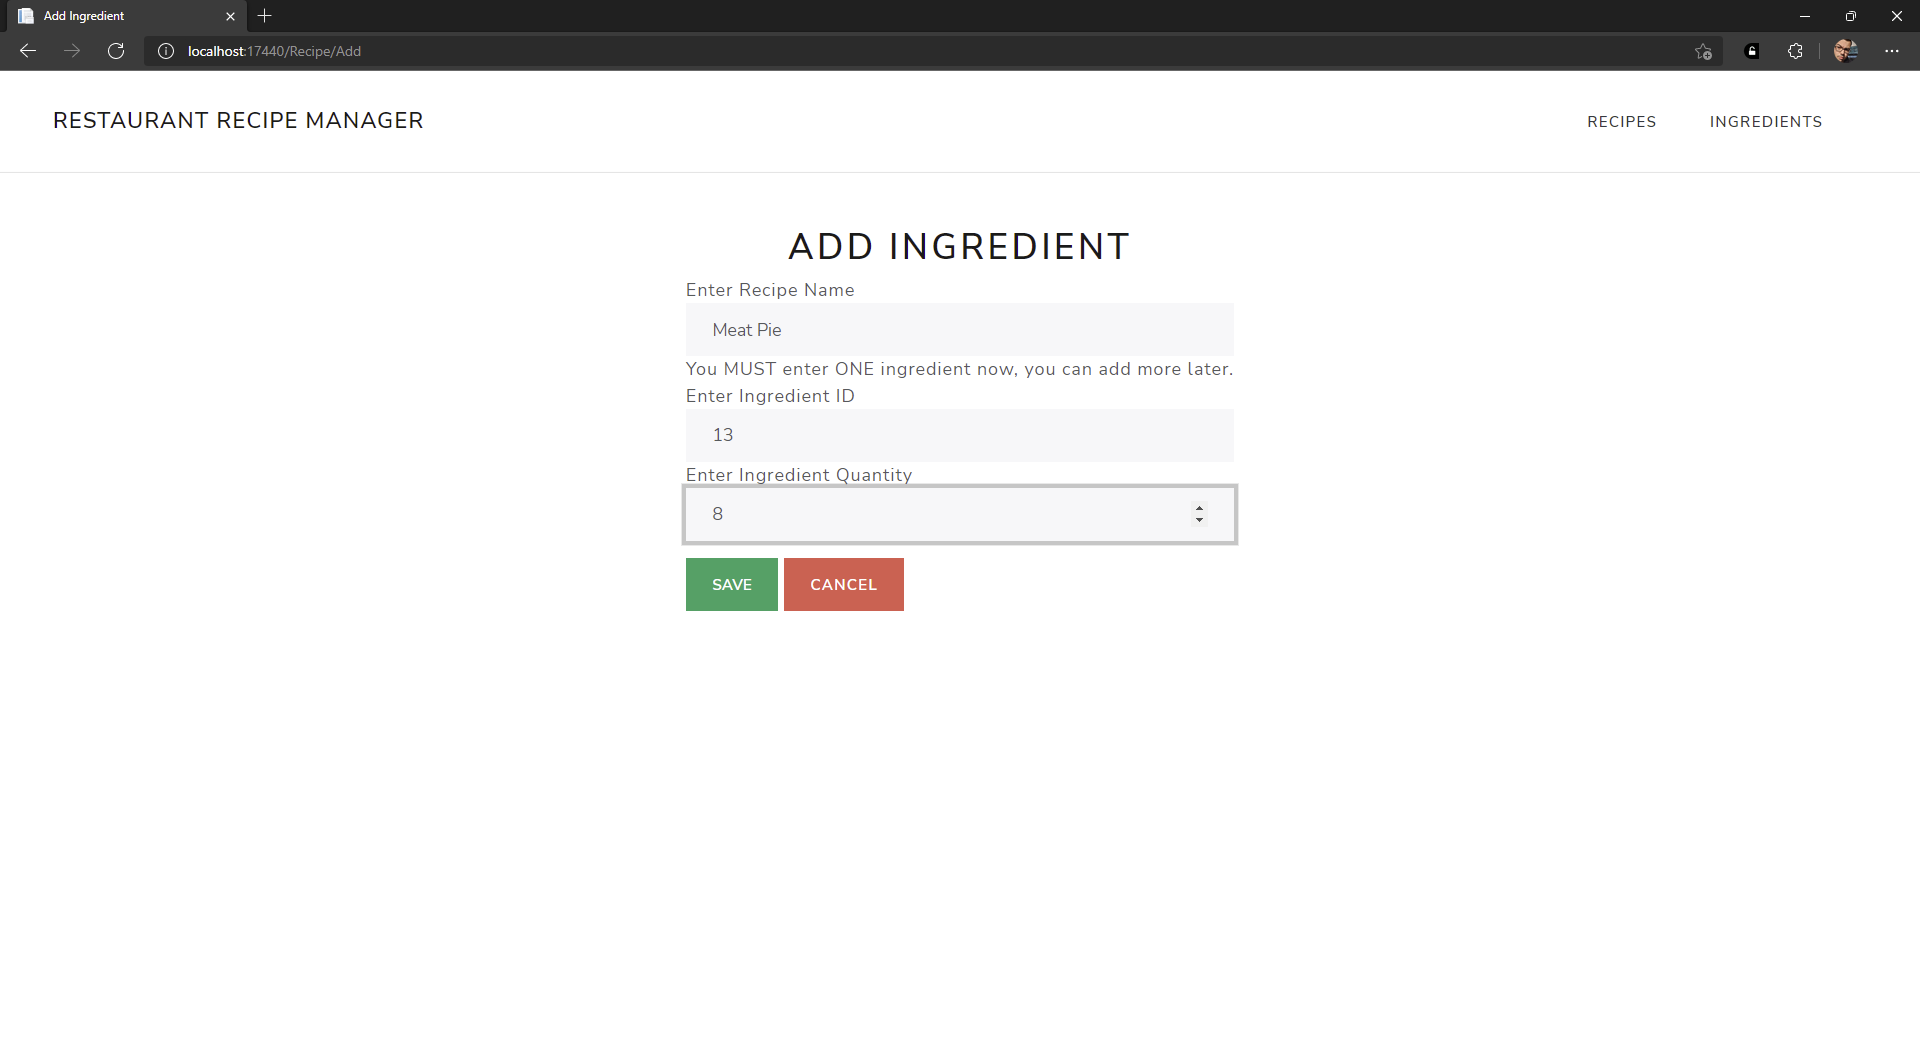
\includegraphics[width=14cm]{Resources/WebApp/Recipes/recipe (13).png}
    \caption{Ilustração da adição da receita de Empada}
    
\end{figure}
\FloatBarrier
\begin{figure}[!hbt]
    \centering
    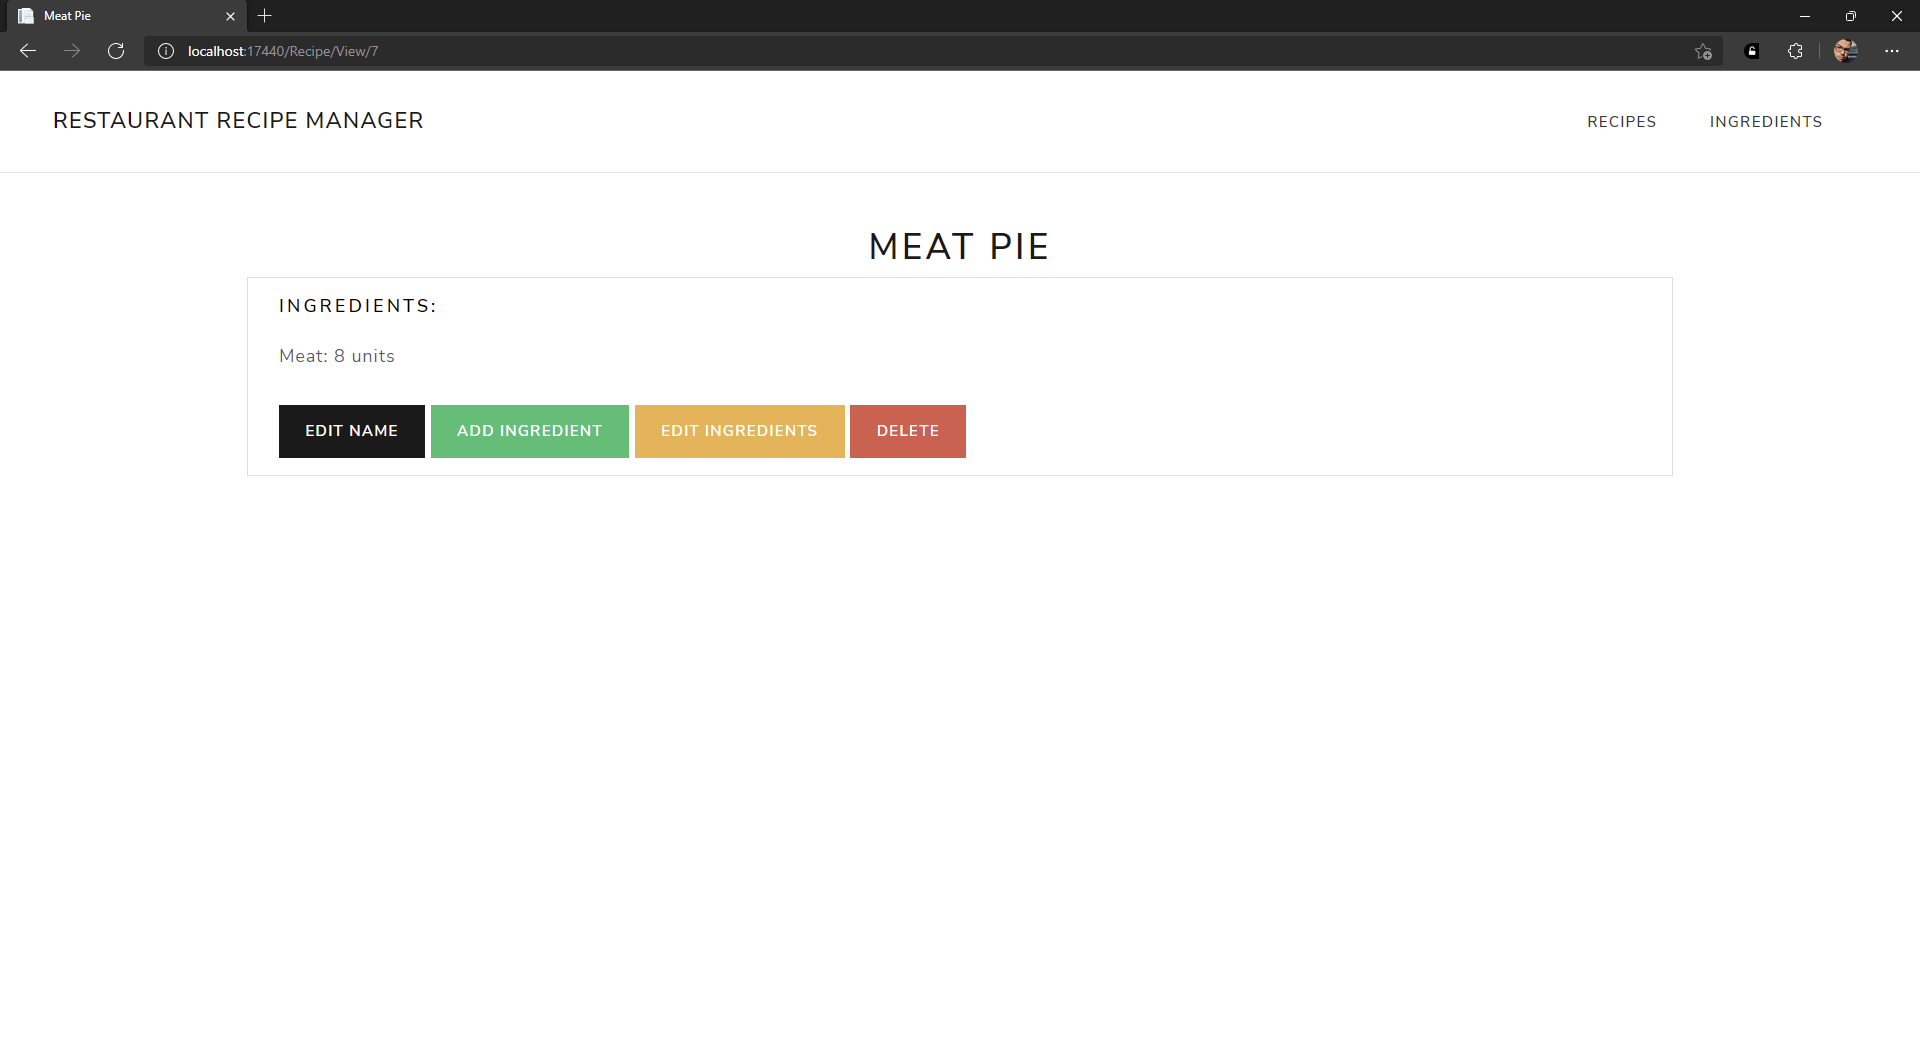
\includegraphics[width=14cm]{Resources/WebApp/Recipes/recipe (14).png}
    \caption{Ilustração da receita de Empada}
    
\end{figure}
\FloatBarrier
\begin{figure}[!hbt]
    \centering
    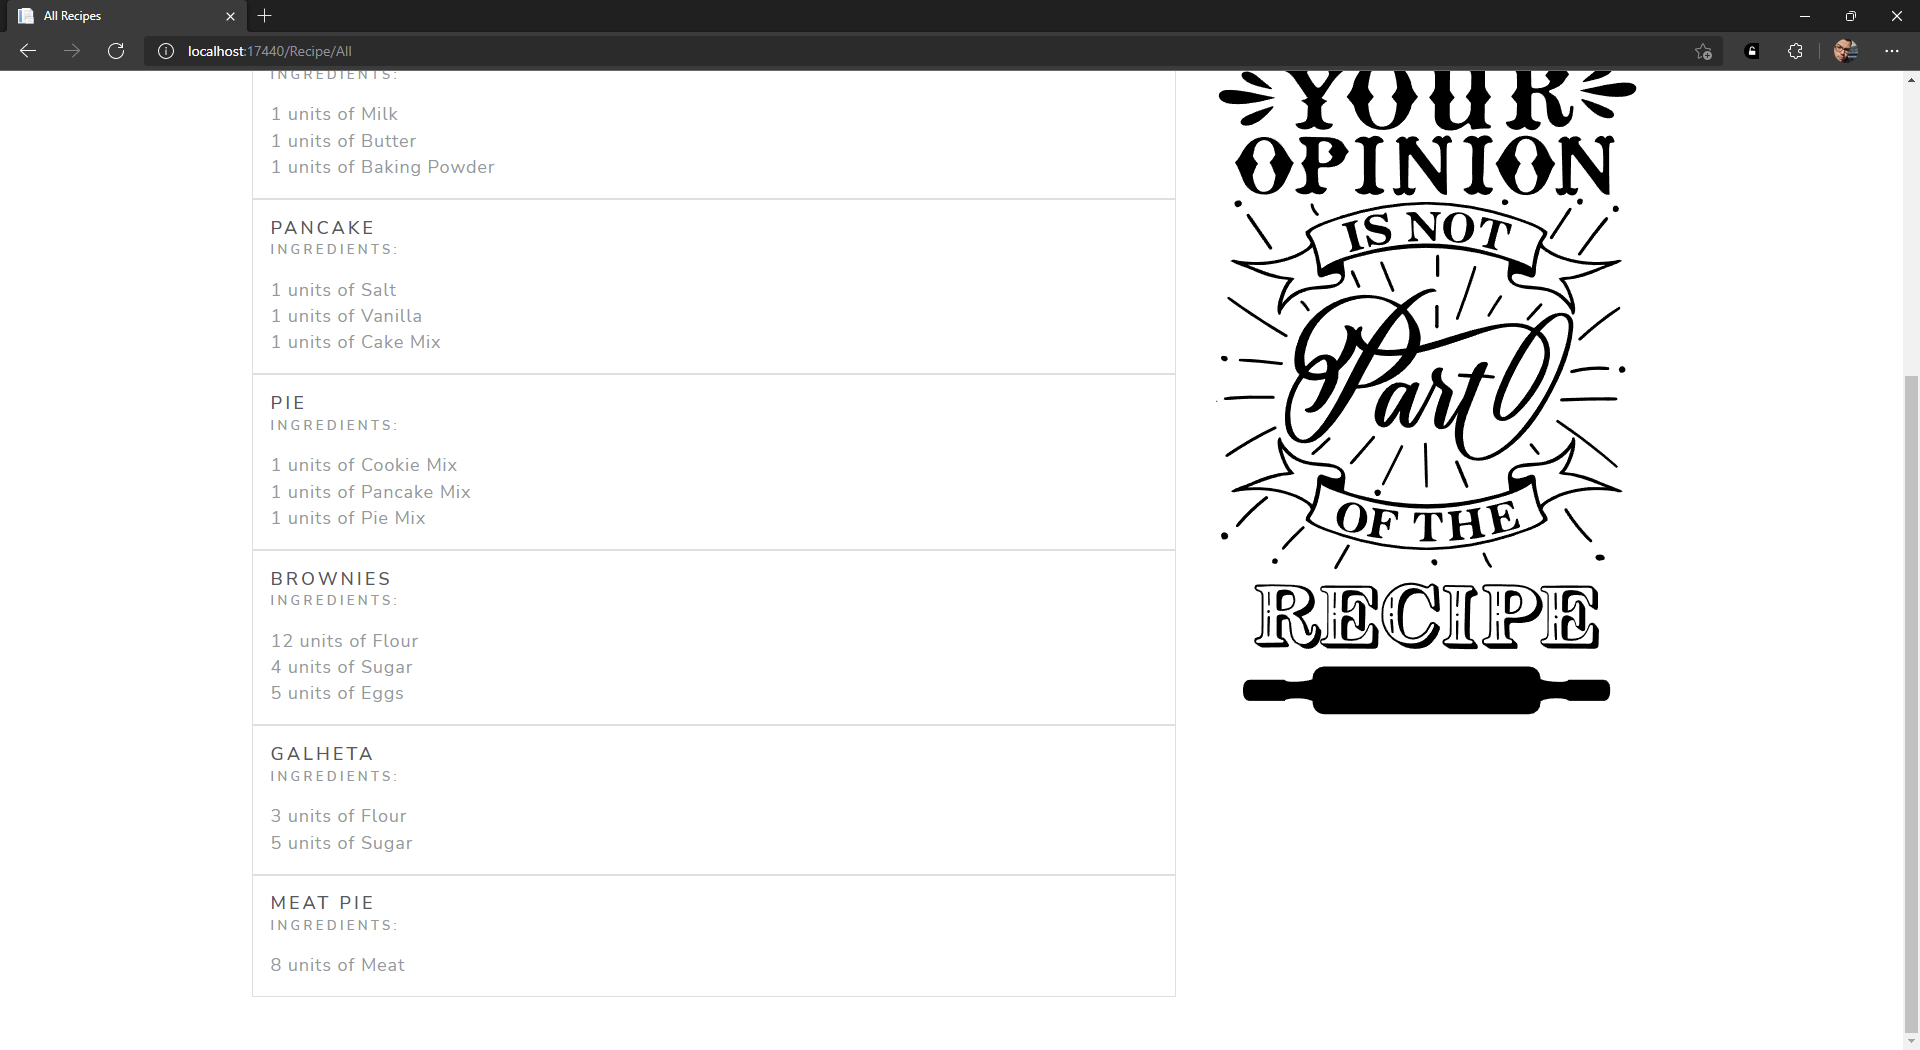
\includegraphics[width=14cm]{Resources/WebApp/Recipes/recipe (15).png}
    \caption{Ilustração da lista de Receitas com a Empada}
    
\end{figure}
\FloatBarrier
\begin{figure}[!hbt]
    \centering
    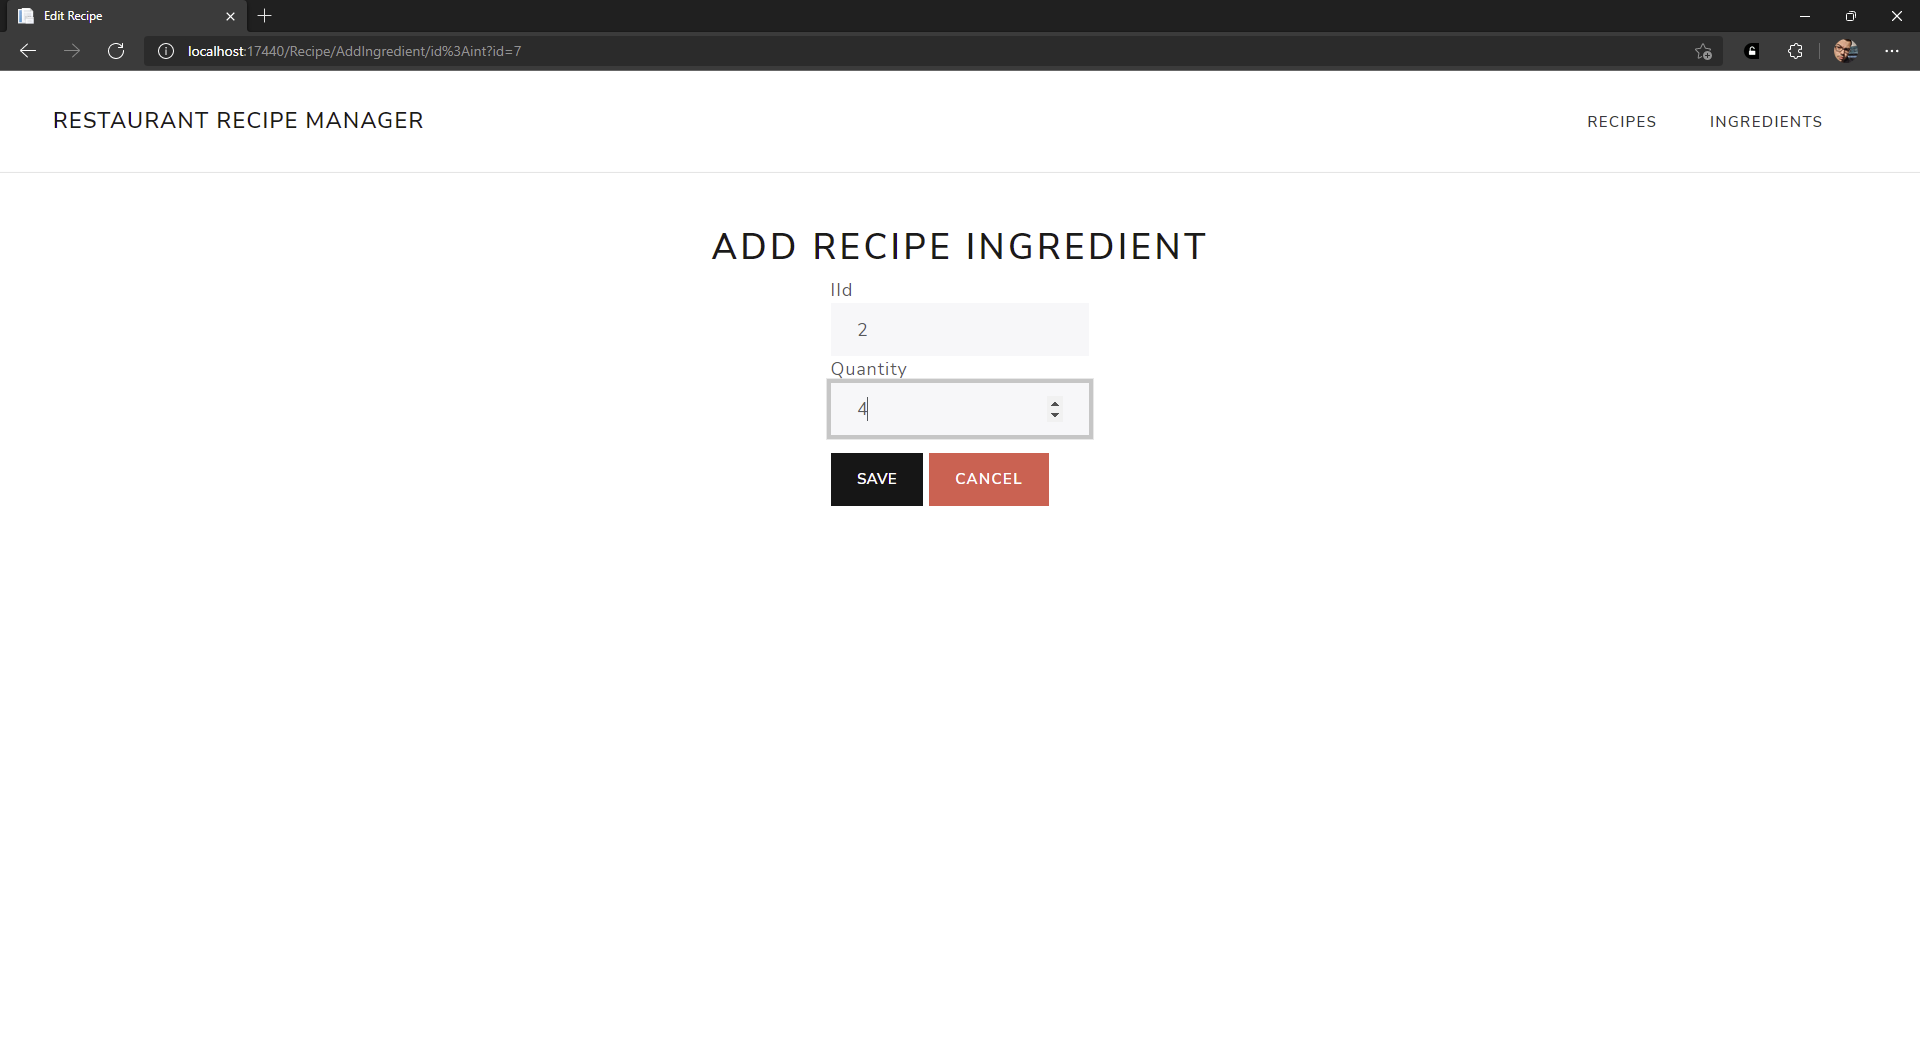
\includegraphics[width=14cm]{Resources/WebApp/Recipes/recipe (16).png}
    \caption{Ilustração da adição de Açúcar à Empada}
    
\end{figure}
\FloatBarrier
\begin{figure}[!hbt]
    \centering
    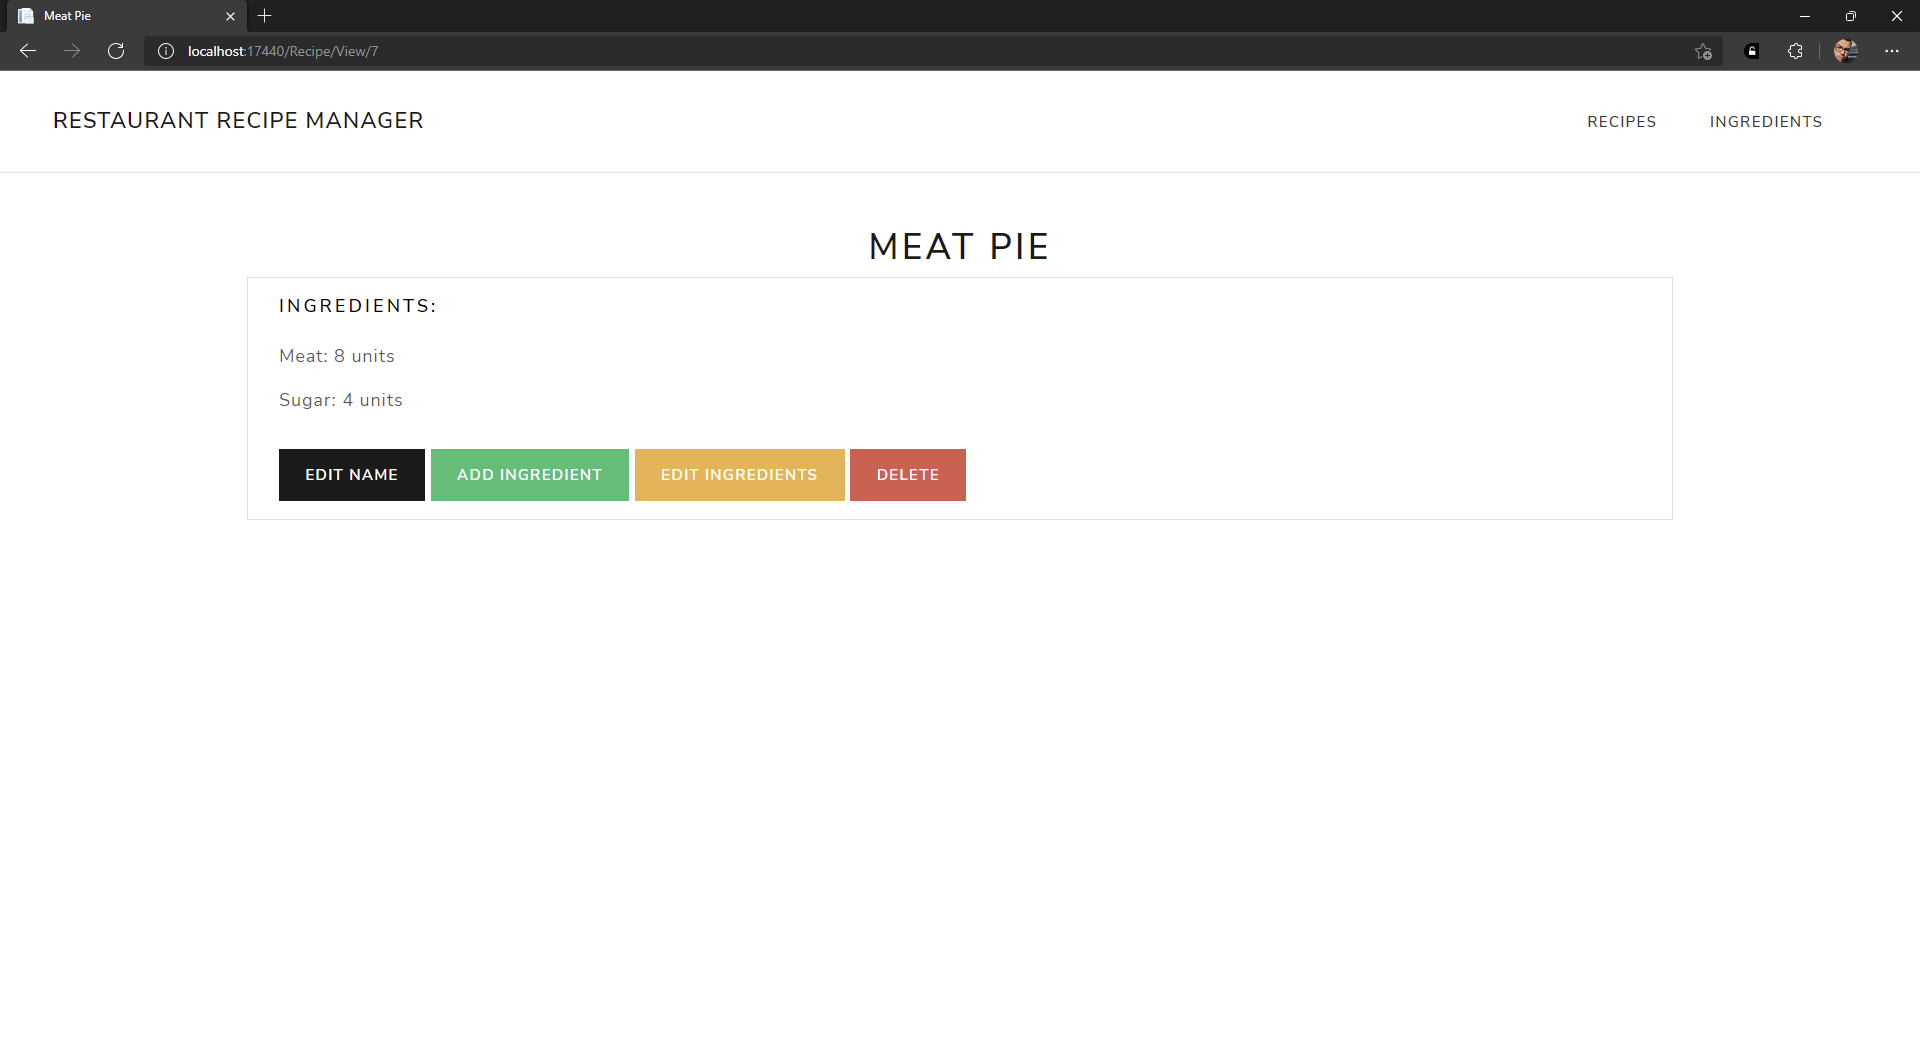
\includegraphics[width=14cm]{Resources/WebApp/Recipes/recipe (17).png}
    \caption{Ilustração da Empada com o Açúcar}
    
\end{figure}
\FloatBarrier
\begin{figure}[!hbt]
    \centering
    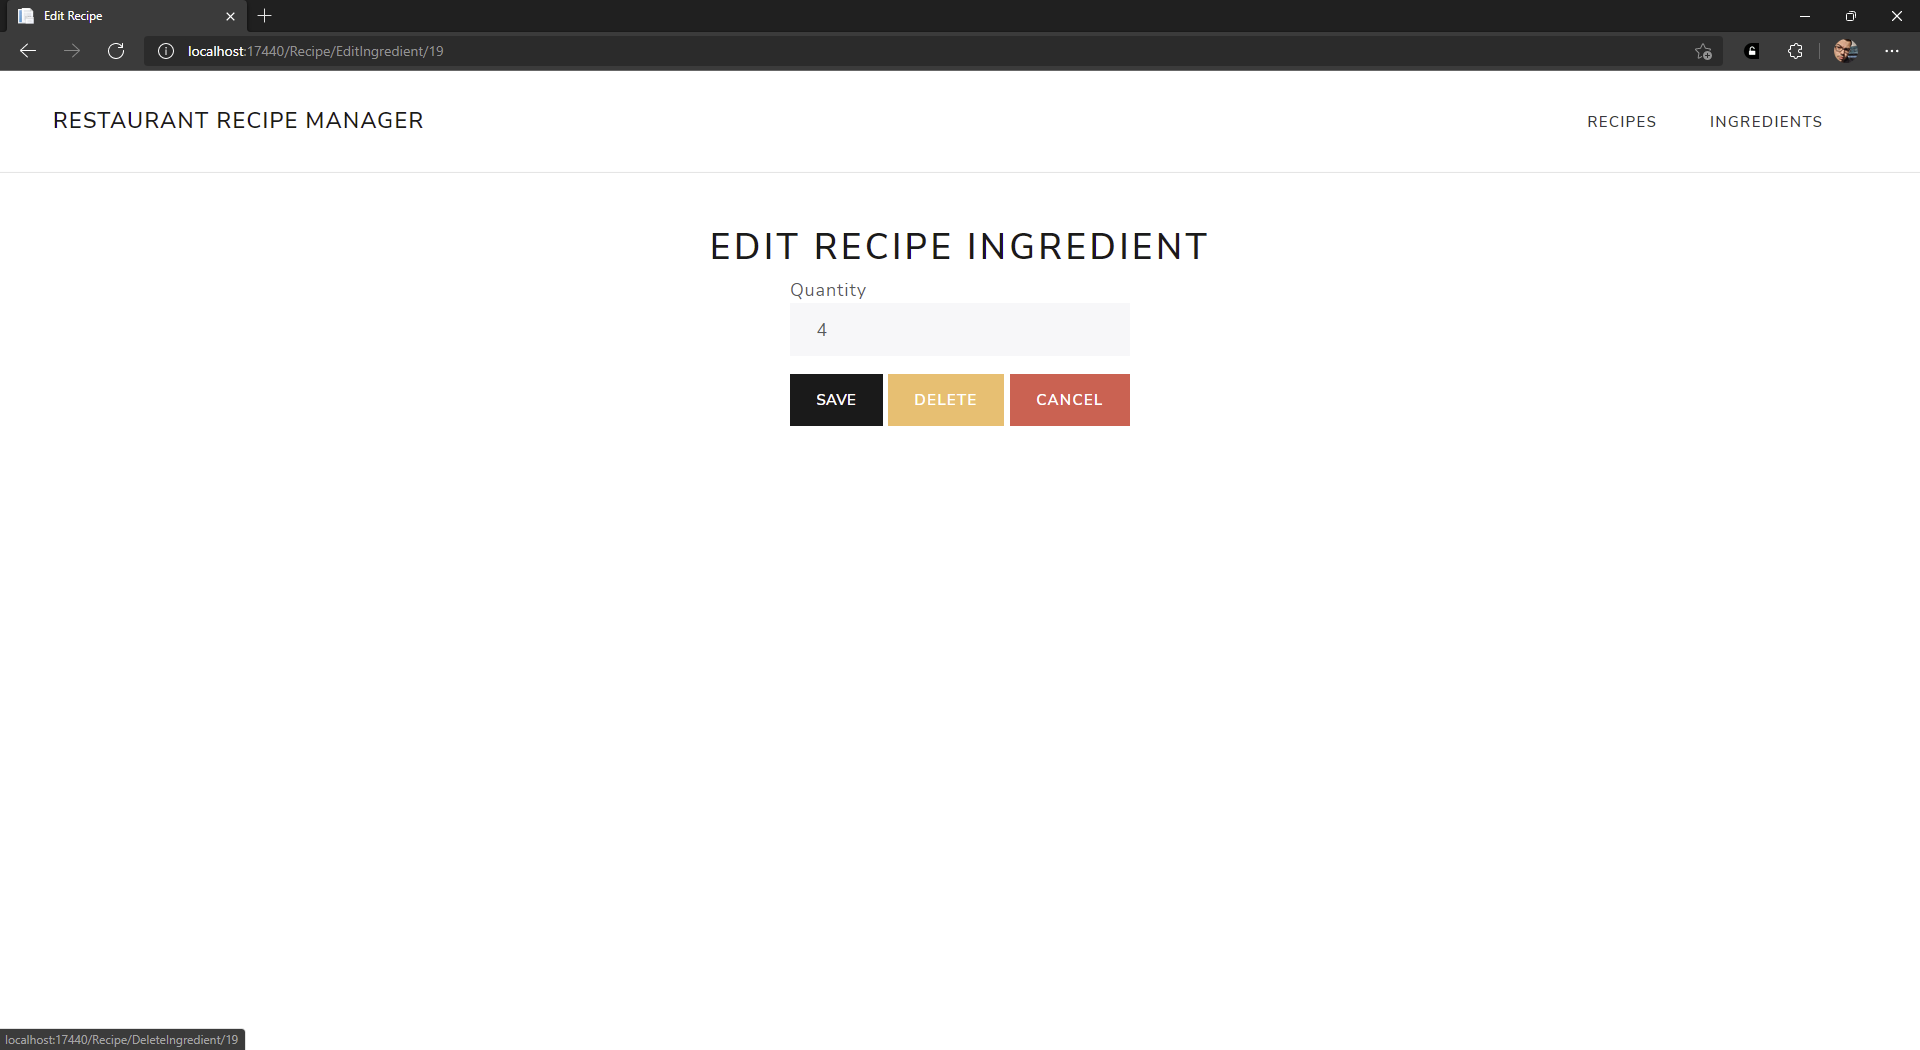
\includegraphics[width=14cm]{Resources/WebApp/Recipes/recipe (18).png}
    \caption{Ilustração da remoção do Açúcar da Empada}
    
\end{figure}
\FloatBarrier
\begin{figure}[!hbt]
    \centering
    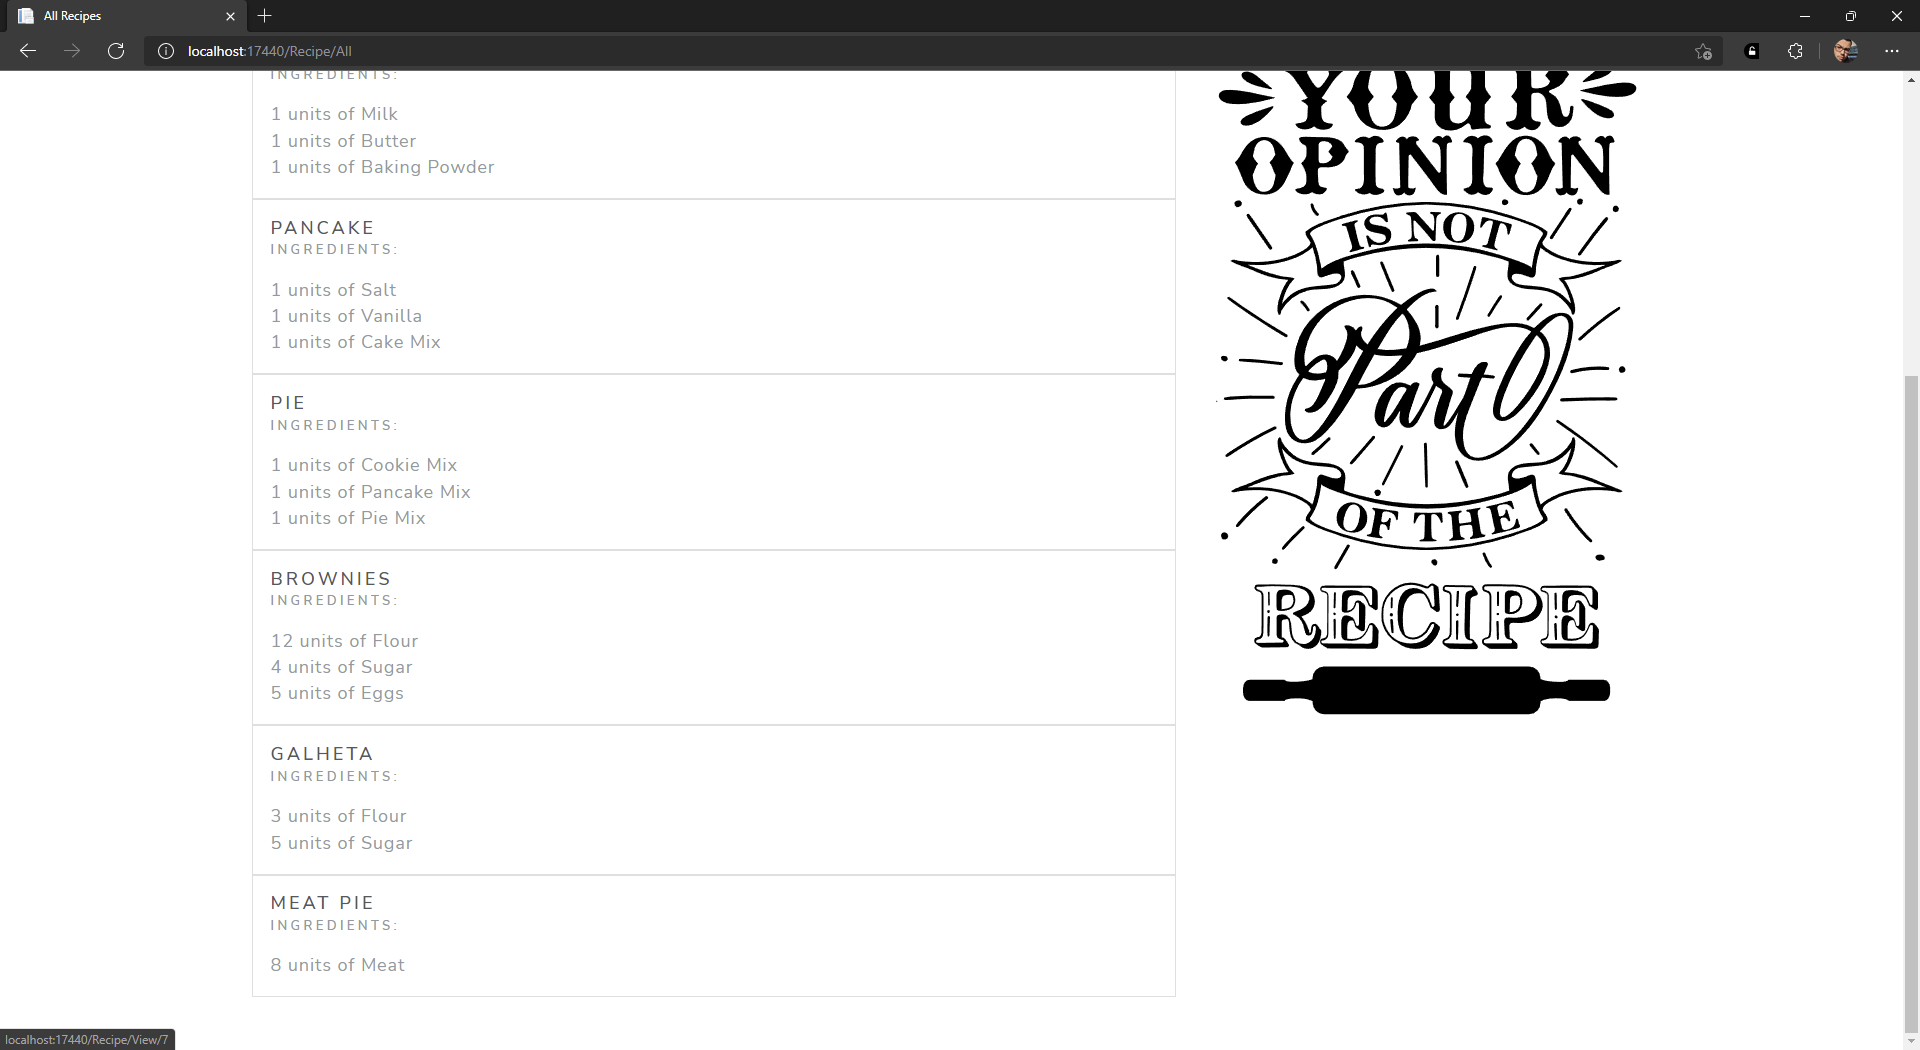
\includegraphics[width=14cm]{Resources/WebApp/Recipes/recipe (19).png}
    \caption{Ilustração da lista com a Empada sem o Açúcar}
    
\end{figure}
\FloatBarrier